\documentclass[10pt,a4paper]{report}
% yeknava

\title{پردازش ابری} %عنوان
\author{یکنوا} %نگارنده

\usepackage[top=35mm, bottom=30mm, left=30mm, right=35mm]{geometry} %تنظیم حاشیه‌های صفحه
\linespread{2.5} %تعداد ۲۲ خط در صفحه

\usepackage{hyperref} %ایجاد لینک در متن
\hypersetup{linkbordercolor={1 1 1}, urlbordercolor={1 1 1}} %سفید کردن مرز لینک‌ها

\usepackage{fancyvrb}
\DefineVerbatimEnvironment{terminal}{Verbatim}{baselinestretch=1} %ایجاد متن‌هایی شبیه به خروجی ترمینال

\usepackage{graphicx} %برای درج شکل در متن

\usepackage{xepersian} %افزودن امکان فارسی نویسی و تعریف قلم‌ها
\settextfont[Scale=1.4]{Nazli}
\setlatintextfont[Scale=1.2]{Ubuntu}
\setdigitfont[Scale=1.4]{B Lotus}
\defpersianfont\Yagut[Scale=1.4]{B Yagut}
\defpersianfont\Yagutb[Scale=1.6]{B Yagut}
\defpersianfont\Titr[Scale=7.2]{Titr}
\defpersianfont\Nazanin[Scale=3.6]{B Nazanin}
\defpersianfont\Titrh[Scale=1.8]{Titr}
\defpersianfont\Titrd[Scale=1.2]{Titr}
\defpersianfont\Titrc[Scale=1.4]{Titr}
\deflatinfont\Titles[Scale=1.6]{Ubuntu}
\deflatinfont\Titlec[Scale=1.4]{Ubuntu}

\makeatletter %شروع به تغییرات در قالب پیش‌فرض برای ایجاد قالب دلخواه
\newcommand\Yagutfont[1]{\def\@yagutfont{#1}}
\newcommand\Yagutfontb[1]{\def\@yagutfontb{#1}}
\newcommand\Titrfont[1]{\def\@titrfont{#1}}
\newcommand\Nazaninfont[1]{\def\@nazaninfont{#1}}



\renewcommand\tableofcontents{% تنظیم مکان و فونت کلمه‌ی فهرست مطالب
\newpage
    \if@twocolumn
      \@restonecoltrue\onecolumn
    \else
      \@restonecolfalse
    \fi
    \centerline{\@yagutfontb\bfseries\contentsname
        \@mkboth{%
           \MakeUppercase\contentsname}{\MakeUppercase\contentsname}}%
    \vskip 40.pt
    \@starttoc{toc}%
    \if@restonecol\twocolumn\fi
}

\renewcommand{\@starttoc}[1]{% درج و تنظیم کلمات عنوان و فهرست
 \begingroup
 \hbox to \textwidth{\@yagutfont\bfseries\underline{صفحه}\hfill\underline{عنوان}}
    \@input{\jobname.#1}%
    \if@filesw
      \expandafter\newwrite\csname tf@#1\endcsname
      \immediate\openout \csname tf@#1\endcsname \jobname.#1\relax
    \fi
    \@nobreakfalse
  \endgroup
}

\def\@spart#1{%
    \addcontentsline{toc}{chapter}
       {\@yagutfont#1}
    \thispagestyle{empty}
    {\centering
     \interlinepenalty \@M
     \@titrfont
     \bfseries #1\par}%
    \@endpart
}

\def\@chapter[#1]#2{\ifnum \c@secnumdepth >\m@ne
                         \refstepcounter{chapter}
                         \typeout{\@chapapp\space\thechapter.}
                         \addcontentsline{toc}{chapter}
                                   {\@yagutfont\@chapapp\space\@tartibi\c@chapter: \normalfont#1}
                    \else
                      \addcontentsline{toc}{chapter}{#1}
                    \fi
                    \chaptermark{#1}
                    \addtocontents{lof}{\protect\addvspace{10.pt}}
                    \addtocontents{lot}{\protect\addvspace{10.pt}}
                    \if@twocolumn
                      \@topnewpage[\@makechapterhead{#2}]
                    \else
                      \@makechapterhead{#2}
                      \@afterheading
                    \fi
}

\def\@makechapterhead#1{
  \thispagestyle{empty}
  \if@twocolumn
    \onecolumn
    \@tempswatrue
  \else
    \@tempswafalse
  \fi
  \vspace*{45mm}
  {\centering
     \interlinepenalty \@M
     \@titrfont
     \ifnum \c@secnumdepth >-2\relax
       \bfseries \chaptername\nobreakspace\@tartibi\c@chapter
       \par
       \vskip 60mm
     \fi
     \@nazaninfont
     \bfseries #1\par}
     \newpage
     \vspace*{50.pt}
     \par
}

\def\@makeschapterhead#1{%
  \vspace*{50.pt}%
  {\parindent \z@ \raggedleft
    \normalfont
    \interlinepenalty\@M
    \@yagutfontb \bfseries  #1\par\nobreak
    \vskip 40.pt
  }
}

\renewcommand\section{\@startsection {section}{1}{\z@\\}
                                   {-8.5ex \@plus -1ex \@minus -.2ex}
                                   {2.3ex \@plus.2ex}
                                   {\@yagutfontb\bfseries}
}

\def\thesection{\arabic{section}-\arabic{chapter})}%

\renewcommand\subsection{\@startsection {subsection}{2}{\z@\\}
                                     {-4.25ex\@plus -1ex \@minus -.2ex}
                                     {1.5ex \@plus .2ex}
                                     {\@yagutfont\bfseries}
}

\def\thesubsection{\arabic{subsection}-\arabic{section}-\arabic{chapter})}%  
%تغییرات برای ایجاد subsubsection
\renewcommand{\subsubsection}{\@startsection{subsubsection}{3}{\z@\\}
                                     {-.25ex\@plus -1ex \@minus -.2ex}
                                     {1.5ex \@plus .2ex}
                                     {\@yagutfont\bfseries}}
\renewcommand{\thesubsubsection}{\arabic{subsubsection}. }
\setcounter{subsubsection}{0}%
\setcounter{secnumdepth}{3}
\setcounter{tocdepth}{3}
\def\thesubsubsection{\arabic{subsubsection}-\arabic{subsection}-\arabic{section}-\arabic{chapter})}% پایان تغییرات برای زیر،زیر فصل
\makeatother %پایان تغییرات در قالب پیش‌فرض برای ایجاد قالب دلخواه
\Yagutfont{\Yagut}
\Yagutfontb{\Yagutb}
\Titrfont{\Titr}
\Nazaninfont{\Nazanin}
\SepMark{-} %استفاده از خط تیره به جای نقطه در فاصله‌گذاری شماره‌های بخش، زیربخش و…
 %اعمال تغییرات گفته شده در آئین‌نامه

\makeatletter%تغییرات دستی برای تنظیم شماره صفحات به صورت ابجد
\def\@myharfi#1{\ifcase#1\or الف\or ب\or پ\or ت\or ث\or
ج\or چ\or ح\or خ\or د\or ذ\or ی\or ز\or س\or ش\or ص\or ض\or ع\or غ\or
ف\or ق\or ک\or گ\or ل\or م\or ن\or و\or ه\or ی\else\@ctrerr\fi}
\def\myharfi#1{\expandafter\@myharfi\csname c@#1\endcsname}
\makeatother

\begin{document} %شروع سند پایان‌نامه
\pagenumbering{myharfi} %شماره‌ی صفحات به صورت الفبایی

\thispagestyle{empty}
\begin{center}
% \vspace{-2cm}\centerline{{\includegraphics[height=3cm]{cover.png}}}
\Titrh اوبونتو برای تازه‌واردها\\
\Yagut نسخهٔ ۱۴/۰۴\\
\par\vspace{29mm}
\Titrc به‌کوشش: \\
\Yagut نوا اژدری \\
\Yagut ساسان نمیرانیان \\
\Yagut احمد صوفی محمودی \\
\par\vspace{29mm}
\Titrc حروف‌چینی: \\
\Yagut احمد صوفی محمودی \\
\Yagut نوا اژدری
\end {center}
\newpage
 %درج صفحه‌ی نخست
\chapter*{مجوز}
\section{متن فارسی}
متن این کتاب تحت مجوز بین‌المللی {\lr{\fontfamily{ptm}\selectfont Creative Commons Attribution-NonCommercial-ShareAlike 4.0}} است. برای دیدن یک رونوشت از این مجوز، به این آدرس بروید:
\begin{LTRitems}
\url{http://creativecommons.org/licenses/by-nc-sa/4.0/}.
\end{LTRitems}
\vspace{1cm}

\section{متن انگلیسی}
{
\lr{
\fontfamily{ptm}\selectfont
This work is licensed under the Creative Commons Attribution-NonCommercial-ShareAlike 4.0 International License. To view a copy of this license, visit 
\begin{LTRitems}
\url{http://creativecommons.org/licenses/by-nc-sa/4.0/}.
\end{LTRitems}
}
}
\vfill
\begin{center}

\includegraphics[scale=0.8]{pics/cc-by-nc-sa.png}
\end{center}

% \include{ThanksGiving} %درج تقدیم‌نامه و صفحه‌ی تقدیر و تشکر
\tableofcontents %چاپ فهرست مطالب
% \listoftables
% \listoffigures
\chapter*{مقدمه}
\emph{\lr{Ubuntu}} تنها یک سیستم عامل آزاد و متن‌باز  با بیش از ۲۰ میلیون کاربر در سرتاسر جهان نیست؛ اوبونتو یک فرهنگ است، یک خلاقیت بزرگ، یک پروژهٔ گروهی، در نوبهٔ خود مهم‌ترین و برجسته‌ترین. اوبونتو یک جامعه از مردم است.\\
اگر در حال خواندن این راهنما هستید، ممکن است تصمیم گرفته باشید که از فضای سیستم عامل‌هایی مانند \lr{Windows} و \lr{Mac OS X} دور شوید و یا شاید اخیراً اوبونتو را بر روی رایانهٔ‌تان نصب کرده‌اید، اما مطمئن نیستید که از کجا باید شروع کنید.\\
استفاده از یک سیستم عامل جدید می‌تواند ترسناک باشد، مخصوصاً وقتی که با کلمه‌های ناآشنا روبه‌رو می‌شوید. بسیاری از مردم با اصطلاحات فنی یک سیستم عامل آشنا نیستند و معتقدند که این مفاهیم برایشان خیلی پیشرفته است. در واقع این موضوع درست نیست. اوبونتو به راحتی نصب می‌شود و استفاده از آن ساده است. و از همه مهم‌تر این‌که: \emph{کاملاً آزاد و  رایگان است}.\\

این راهنما برای کسانی است که به تازگی استفاده از گنو/لینوکس را شروع کرده‌اند و این امکان را به آن‌ها می‌دهد که تمام ابزارهای موردنیاز را بشناسند و از آن‌ها به درستی استفاده کنند.\\
شما با خواندن این کتاب می‌آموزید که چگونه کارهای زیر را انجام دهید:
\begin{itemize}
\item نصب و راه‌اندازی اوبونتو بر روی رایانه‌ٔتان
\item پشتیبانی فنی در این محیط
\item درک فلسفهٔ اوبونتو
\item ایجاد وحدت در رابط میز کاربری
\item استفاده از نرم افزارهای سازگار با اوبونتو
\end{itemize}
 %درج مقدمه

\newpage %رفتن به صفحه‌ی جدید برای پایان دادن به شماره‌گذاری الفبایی صفحات

\pagenumbering{arabic} %شماره‌ی صفحات به صورت عددی

\chapter{معرفی اوبونتو}
قبل از اینکه شروع به نصب کنیم، بهتر است در مورد فلسفه و مفهوم کلی سیستم‌عامل اوبونتو صحبت کنیم.
\section{تعاریف کلی}
بهتر است قبل از پرداختن به اوبونتو، در مورد برخی تعاریف، مثل سیستم‌عامل و هسته، توضیح داده شود.
\subsection{سیستم‌عامل چیست؟}
سیستم‌عامل برنامه‌ای است که با سخت‌افزار ارتباط مستقیم دارد و امکان اجرای برنامه‌های کاربردی (\lr{Application}) را روی بستر سخت‌افزاری ممکن می‌سازد.
\subsection{هسته چیست؟}
هسته نقش قسمت مرکزی و سطح پایین یک سیستم‌عامل را ایفا می‌کند و وظایفی مانند ارتباط با سخت‌افزار و بارگذاری درایورها را به دوش می‌کشد.
\subsubsection{لینوکس چیست؟}
برخلاف تصور خیلی از افراد، لینوکس تنها یک هسته با همان وظایف گفته شده است. بسیار کم پیش می‌آید که در کاربرد روزانه، به طور مستقیم با خود هستهٔ لینوکس ارتباط برقرار کنیم. با این حال، هسته نقش اصلی را در سیستم‌عامل بر عهده دارد.
\subsubsection{چرا گنو/لینوکس آری، لینوکس نه؟}
همان طور که گفته شد، لینوکس تنها یک هسته است و یک هسته به خودی خود هیچ کاری نمی‌تواند برای ما انجام دهد. ما برای برطرف‌کردن نیازهای روزانه به نرم‌افزارهای متعددی نیازمندیم. نرم‌افزارهایی که اکثراً از پروژهٔ گنو گرفته شده یا بر اساس فلسفهٔ نرم‌افزارهای آزاد و مجوز \lr{GNU GPL} ساخته شده‌اند. برای همین، بهتر است این سیستم‌عامل (و نه خود هسته) را گنو/لینوکس بنامیم.
\subsubsection{توزیع گنو/لینوکس چیست؟}
گفتیم که پروژهٔ گنو/لینوکس از پیوستن ابزارهای گنو و هستهٔ لینوکس به وجود آمد. حالا فرض کنید که بخواهید آن را نصب کنید. چکار باید بکنید؟ در حالت قدیمی، باید یک متخصص کامل یونیکس باشید: هسته را بگیرید و کامپایل کنید، بعد یک دیسک را فرمت کنید و بوت سکتور را طوری تنظیم کنید که از این کرنل بوت شود. سپس دستورات (برنامه‌های) دیگر را روی آن کپی کنید و تمام وابستگی‌ها را هم رعایت کنید. چنین کاری برای بیش‌تر کاربران بسیار سخت است.\\
برای حل این مشکل، افراد و شرکت‌هایی آمده‌اند و توزیع‌هایی (\lr{Application}) را ساخته‌اند. در همان سال ۱۹۹۲ که هستهٔ لینوکس آمد، توزیع‌ها هم ظاهر شدند. کاربران هسته را به همراه چند برنامه اصلی و یک برنامه نصب کننده روی یکی دو فلاپی جا می‌دادند و بین دیگران پخش می‌کردند.
\section{اوبونتو چیست؟}
اوبونتو (تلفظ به صورت \lr{|oo'boontoo|}) یک سیستم‌عامل کاملِ گنو/لینوکسی برای استفاده رومیزی است. اوبونتو (مثل سایر گنو/لینوکس‌ها) آزاد است و دارای پشتیبانی از طرف جامعهٔ کاربری و پشتیبانی حرفه‌ای از طرف شرکت سازندهٔ آن، \lr{Canonical}، است.\\
\subsection{چطور اوبونتو  و لینوکس به هم مربوط‌اند؟}
اوبونتو یک سیستم‌عامل است که از لینوکس به عنوان هسته استفاده می‌کند. به طور ساده، لینوکس یک بخش از اوبونتو  است که وظیفهٔ مرکزی را به عهده دارد.\\

جامعهٔ اوبونتو بر پایهٔ اندیشه‌های مطرح‌شده در بیانیهٔ اوبونتو فراهم آمده است. این‌که:

\begin{itemize}
\item نرم‌افزار باید رایگان باشد.
\item نرم‌افزارها باید در زبان محلی کاربران قابل استفاده باشند و معلولیت‌ها را هم پوشش دهد تا اوبونتو برای بیش‌ترین افراد ممکن مورد استفاده قرار گیرد.
\item کاربران باید آزادی تغییر نرم‌افزار به شیوهٔ دلخواه‌شان را داشته باشند.\\
\end{itemize}

برای همین، اوبونتو تنها یک سیستم‌عامل نیست و دارای سه بخش متفاوت است:

\begin{itemize}
\item فلسفه
\item پروژهٔ نرم‌افزار مشترک جهانی
\item سیستم‌عامل
\end{itemize}

این راهنما در تمام این مفاهیم در بخش‌های بعد گسترده می‌شود؛ اما در حال حاضر، مهم‌ترین چیز که باید به خاطر داشته باشید این است که اوبونتو بیش‌تر از یک نرم افزار است.

\section{فلسفهٔ اوبونتو}
اوبونتو یک لغت قدیمی در زبان آفریقایی به معنای «یک نفر برای همه» یا «انسانیت با دیگران» است.\\
مجموعهٔ اوبونتو با سیستم‌عامل‌های دیگر متفاوت است، به دلیل اینکه روح انسانیت و جامعه را به دنیای رایانه می آورد. کاربران اوبونتو در یک باور عمیق هم‌عقیده‌اند که نرم‌افزار باید قابل دسترس برای همهٔ انسان‌ها، با هر زبان و رنگ پوست، توانایی جسمانی و درآمدی باشد.

\section{نرم‌افزار اختصاصی در مقابل نرم‌افزار آزاد و متن‌باز}
نرم‌افزارهای اختصاصی توسط یک شرکت طراحی می‌شوند، توسعه می‌یابند و فروخته می‌شوند. این نرم‌افزارها برای به‌دست‌آوردن سود فروخته می‌شوند و اکثراً فقط بر روی یک نوع از کامپیوترها کاربرد دارند. برای مثال، سیستم‌عامل‌های اختصاصی مانند \lr{Microsoft Windows} و یا \lr{Mac OS X} را در نظر بگیرید. کد منبع این سیستم‌ها در دسترس نیست و اگر شما سعی به تغییر یا توزیع آن را داشته باشید، متهم خواهید شد.\\
اوبونتو، به عبارت دیگر، یک نرم افزار اختصاصی نیست؛ به این دلیل که به صورت فعال توسط جامعهٔ \lr{FOSS} نگهداری می شود.

\subsection
{
\lr{FOSS}
چیست؟
}

\lr{FOSS} مخفف عبارت \lr{Free/Libre Open Source Software} و به معنی نرم‌افزار آزاد و متن‌باز است. نرم‌افزار \lr{FOSS} به دلایل زیر با نرم‌افزارهای اختصاصی تفاوت دارد:

\begin{itemize}
\item استفادهٔ آزاد و رایگان
\item اشتراک‌گذاری آزاد و رایگان
\item توسعهٔ آزاد و رایگان
\end{itemize}

این یعنی شما بدون پرداخت هیچ مبلغی می‌توانید اوبونتو را دانلود و استفاده کنید. شما می‌توانید به صورت کاملاً قانونی از سی‌دی/دی‌وی‌دی های اوبونتو به هر تعداد که می‌خواهید، کپی کرده و بین دوستان و آشنایان‌تان توزیع کنید. حتا کد منبع سیستم‌عامل اوبونتو آزادانه در دسترس شماست و می‌توانید آن را با توجه به نیازهای خود تغییر دهید.\\
اوبونتو از مجوز عمومی همگانی \lr{GNU}  (یا به طور ساده \lr{GPL}) استفاده می‌کند که به طور گسترده در جامعهٔ \lr{FOSS} استفاده می‌شود. به همین دلیل، اوبونتو دارای آزادی‌هایی است که ذکر شد.\\
\lr{GPL} توسط بنیان‌گذار پروژهٔ گنو و بنیاد نرم‌افزارهای آزاد، ریچارد استالمن، در سال ۱۹۸۹ نوشته شد و در آن به صراحت آمده است که کاربران برای اجرا، کپی، توزیع ، بازرسی، تغییر ، توسعه و بهبود نرم‌افزار ارائه‌شده آزاد هستند. گاهی \lr{GPL} با  نام مستعار کپی‌لفت (\lr{Copyleft}) می‌آید.

\subsection{چطور ممکن است اوبونتو رایگان باشد؟}
شما ممکن است تعجب کنید که در حال حاضر واقعاً چطور ممکن است اوبونتو رایگان باشد. آیا نکته و یا برخی هزینه‌های مخفی وجود دارد؟ به دو دلیل اوبونتو رایگان است.\\
\begin{enumerate}
\item \textbf{مدیریت و بودجه‌بندی به پشتوانهٔ کنونیکال}\\
اگر چه  اوبونتو توسط جامعهٔ \lr{FOSS} نگهداری می‌شود، ولی مدیریت و تأمین بودجه از طریق شرکت خصوصی کنونیکال انجام می‌شود.\\
کنونیکال پشتیبانی‌های تجاری را برای شرکت‌ها تامین می‌کند و از این راه درآمد دارد. درآمد حاصل از این پشتیبانی، برای توسعهٔ مستمر اوبونتو مصرف می‌شود. این توسعهٔ مستمر، شامل موارد زیر است:
\begin{itemize}
\item انتشار نسخه‌های جدید اوبونتو هر شش ماه یک‌بار
\item به‌روزآوری‌های امنیتی
\item سرورهای میزبانی وب برای جامعهٔ آنلاین اوبونتو 
\item دفاتر کنونیکال
\end{itemize}
\item \textbf{اوبونتو از طریق جامعهٔ \lr{FOSS} نگهداری می‌شود}\\
از آنجایی که اوبونتو نرم‌افزاری کدباز است، کاربران برای دسترسی و تغییر کد منبع آزاد هستند و این به بهترشدن سیستم‌عامل برای همه کمک می‌کند.\\
اوبونتو هم یک جامعهٔ جهانی است و هم یک پروژهٔ نرم‌افزاری مشترک. مردم در سرتاسر جهان می‌توانند زمان و توانایی‌های خود را با هم به اشتراک بگذارند و در فعالیت‌هایی مانند زیر کمک کنند:
\begin{itemize}
\item تست اشکالات نرم‌افزار
\item ارسال مستندات کاربری
\item طراحی اثر هنری
\item ارائهٔ بازخورد
\item نگارش جملاتی زیبا دربارهٔ اوبونتو
\end{itemize}
\end{enumerate}

\section{چرا باید از اوبونتو استفاده کرد؟}
\begin{itemize}
\item[-] کار با اوبونتو ساده است.
\item[-] نصب نرم‌افزار، به‌روزرسانی سیستم‌عامل و پیدا کردن ابزارهای جدید با چند کلیک انجام پذیر است.
\item[-] محیط اصلی اوبونتو که یونیتی نام دارد، بسیار زیباست.
\item[-] آزاد است و برای همیشه رایگان باقی می‌ماند.
\item[-] اوبونتو با مشارکت کاربران‌اش ساخته شده و هرکسی می‌تواند برای بهتر شدن‌اش قدمی بردارد.
\item[-] اوبونتو از هستهٔ لینوکس استفاده می‌کند که طراحی بسیار منطقی و امنی دارد.
\item[-] اوبونتو به طور معمول ویروس نمی‌گیرد.
\item[-] اوبونتو با اکثر رایانه‌ها و لپتاپ‌ها کار می‌کند و در بیش‌تر مواقع حتی نیاز به نصب یک درایور هم ندارید.
\item[-] با برنامه و فایل‌های فعلی‌تان سازگار است. اکثر محتوای چندرسانه‌ای در اوبونتو قابل پخش است و بسیاری از برنامه‌ها، مثل فایرفاکس، کروم و اسکایپ، نسخه‌ای مناسب اوبونتو دارند.
\item[-] از بسیاری از زبان‌ها، از جمله زبان فارسی، به خوبی پشتیبانی می‌کند.
\item[-] پایدار و سرعت آن بالاست. اوبونتو کند نمی‌شود و لازم نیست هر چند وقت دوباره نصب‌اش کنید. به چندین گیگابایت رَم هم برای اجرا نیاز ندارد.
\item[-] همیشه کسی برای کمک هست. اوبونتو در میان فارسی‌زبانان هم شناخته شده است و افراد زیادی در انجمن فارسی اوبونتو و کانال \lr{IRC} اوبونتوی فارسی، بدون هیچ چشم‌داشتی، به شما کمک می‌کنند.

\end{itemize}

\section{نکاتی در مورد اوبونتو}
کنونیکال نسخه‌های جدید اوبونتو را هر شش ماه یک بار، در ماه‌های آوریل و اکتبر، منتشر می‌کند. هر اوبونتو که منتشر می‌شود، یک شماره‌نسخه دارد که از سال و ماه انتشار آن تشکیل شده است. این راهنما به طور عمده برای اوبونتو ۱۴/۰۴ نوشته شده که در ماه آوریل سال ۲۰۱۴ منتشر شده است.
علاوه بر شماره، هر نسخه اوبونتو یک نام هم دارد که از ترکیب یک صفت و نام یک حیوان تشکیل می‌شود. برای مثال نام کد برای اوبونتو ۱۴/۰۴، \lr{Trusty Tahr} است.\\ همچنین اوبونتو ۱۴/۰۴ یک نسخهٔ \lr{LTS} است. \lr{(Long Term Support) LTS} ها نسخه‌هایی از اوبونتو هستند که تقریباً هر دو سال یک‌بار (طبق زمان‌بندی) منتشر می‌شوند و برای ۵ سال بعد از آن پشتیبانی می‌شوند. نسخه‌های عادی ۹ ماه پشتیبانی دارند.\\
 %درج فصل نخست
\chapter{نصب اوبونتو}
\section{دانلود و آماده‌سازی اولیه}
در این قسمت، با توجه به مشخصات سیستم خود، بین نسخهٔ ۳۲ بیتی و ۶۴ بیتی نسخهٔ مناسب با معماریِ کامپیوترتان را از \href{http://www.ubuntu.com/download/desktop}{وب‌گاه اوبونتو} دانلود کنید. بعد از اتمام دانلود، ۲ روش برای نصب دارید: نصب از روی 
\lr{DVD} یا \lr{USB}.

\subsection[نحوهٔ رایت روی DVD]{نحوهٔ رایت روی \lr{DVD}}
بعد از دانلود \lr{ISO} ی مناسب، آن را روی یک دیسک نوری خام بنویسید. 
سیستم‌عامل‌های مختلف ابزارهای متفاوتی برای این کار دارند.

\subsubsection{در ویندوز}
در ویندوز می‌توان از \href{http://infrarecorder.org/}{\lr{InfraRecorder}} 
استفاده کرد.

\subsubsection{در \lr{Mac OS X}}
این سیستم‌عامل به صورت پیش‌فرض ابزار \lr{Disk Utility} را دارد که در مسیر:
\begin{center}
\lr{Disk Utility} \textsf{→} \lr{Utilities} \textsf{→} \lr{Applications}\\
\end{center}
قابل دسترس است. ابزار \lr{Disk Utility} را اجرا و \lr{ISO} را به قاب سمت چپ 
بکشید. بعد از زدن تیک \lr{Verify burned data}، روی \lr{Burn} کلیک کنید.

\subsubsection{در گنو/لینوکس}
کاربران گنو/لینوکس نیز می‌توانند از \lr{Brasero} یا \lr{K3b} استفاده کنند.

\subsection[نحوهٔ نصب بر روی USB]{نحوهٔ نصب بر روی \lr{USB}}
\subsubsection{در ویندوز}
می‌توان از \href{http://www.pendrivelinux.com/}{\lr{Pen Drive Linux}} یا 
\href{http://www.linuxliveusb.com/}{\lr{LiLi}} استفاده کرد. کار با این ابزارها 
بسیار ساده است. نوع توزیع (اوبونتو) و محل فایل \lr{ISO} دانلود شده را به 
نرم‌افزار بدهید و درایو حافظهٔ فلش را مشخص کنید.

\begin{center}
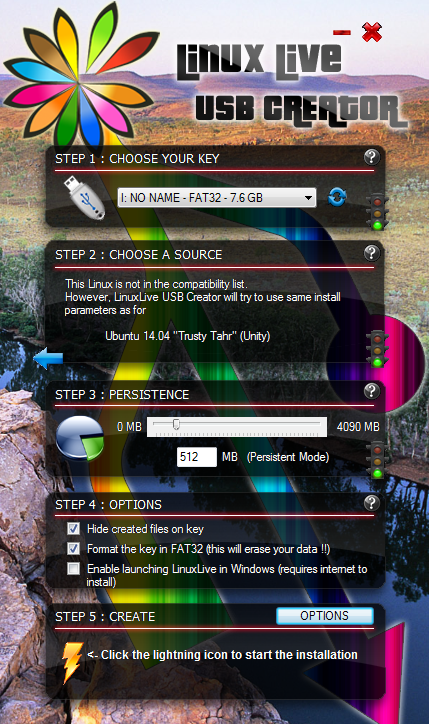
\includegraphics[scale=0.6]{pics/1.png}\\
\end{center}

\subsubsection{در \lr{Mac OS X}}
به کاربران \lr{OS X} توصیه می‌شود که از \lr{CD} یا \lr{DVD} استفاده کنند. زیرا 
رایانهٔ \lr{OS X} آن‌ها قابلیت راه‌اندازی از راه فایل‌های \lr{ISO} را ندارد.

\subsubsection{در گنو/لینوکس}
می‌توان از \lr{Unebootin} (روی تمام توزیع‌ها) و یا \lr{Ubuntu Startup Disk 
Creator} (مخصوص اوبونتو) استفاده کرد.

\begin{center}
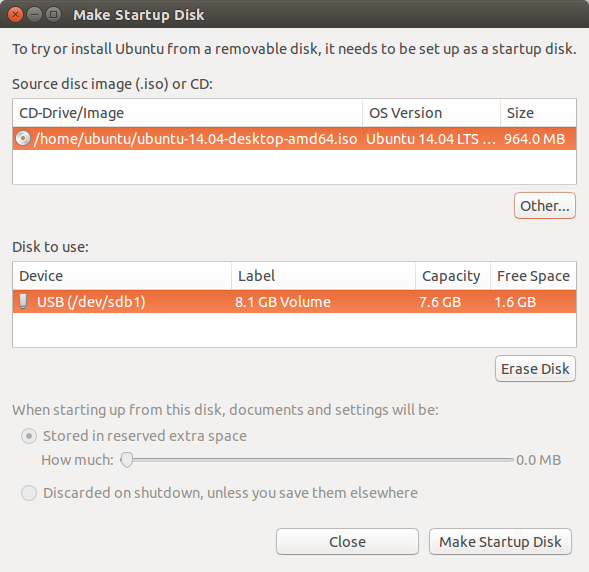
\includegraphics[scale=0.6]{pics/2.png}\\
\end{center}

\section{نصب و راه‌اندازی}
بعد از ریختن اوبونتو روی \lr{DVD} یا \lr{USB}، باید آن را بوت کنید. برای 
بوت‌کردن از راه دی‌وی‌دی یا یواس‌بی، باید به دفترچهٔ مادربورد رایانهٔ‌تان مراجعه 
کنید یا در اینترنت جست‌وجو کنید.\\
بعد از اینکه رایانه را با اوبونتو بوت کردید، دو انتخاب پیش‌رو دارید: انتخاب اول، 
نصب اوبونتو و انتخاب دوم، امتحان‌کردن اوبونتو است. با انتخاب گزینهٔ دوم، شما در 
هر زمان که تمایل به نصب داشتید می‌توانید با کلیک بر روی آیکون نصب اوبونتو آن را 
نصب کنید.
\begin{center}
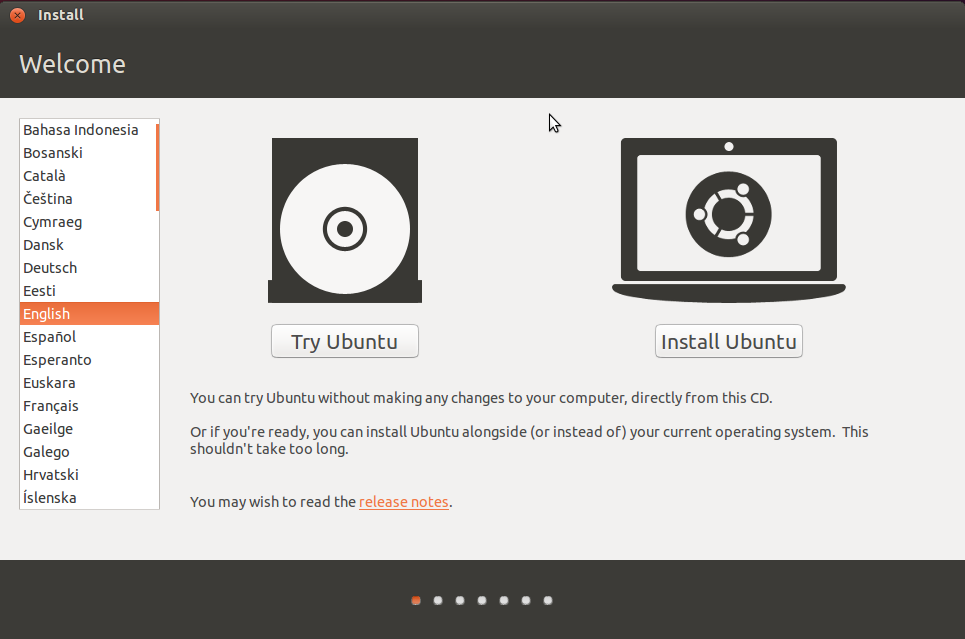
\includegraphics[scale=0.47]{pics/3.png}\\
\end{center}
در گام بعد، در صورتی که به اینترنت وصل نشده باشید و رایانهٔ‌تان دارای کارت شبکهٔ 
بی‌سیم باشد، شبکه‌های بی‌سیم موجود به شما نشان داده می‌شود که می‌توانید از 
همان‌جا شبکهٔ موردنظرتان را انتخاب کنید و به آن وصل شوید.
\begin{center}
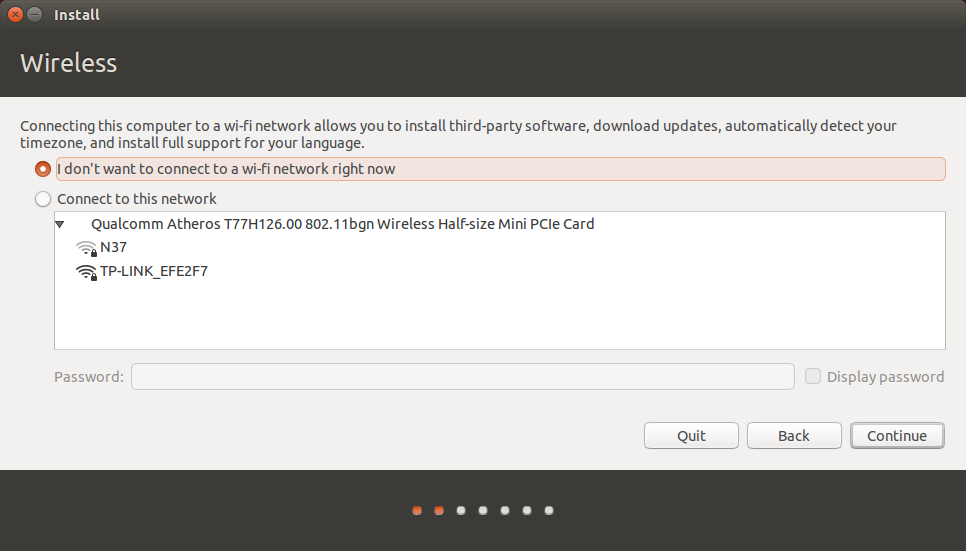
\includegraphics[scale=0.47]{pics/4.png}\\
\end{center}

در مرحلهٔ سوم، اطلاعاتی کلی مثل میزان فضای خالی سیستم‌تان و وصل‌بودن به اینترنت 
یا منبع برق را به شما نشان می‌دهد. همچنین در این مرحله می‌توانید با زدن تیک 
گزینهٔ \lr{Download updates while installing} آخرین به‌روزرسانی‌های اوبونتو را 
ضمن نصب دریافت و نصب کنید و با انتخاب \lr{Install this third-party software} 
کُدک‌های لازم برای پخش فایل‌های \lr{MP3} را نصب کنید.

\begin{center}
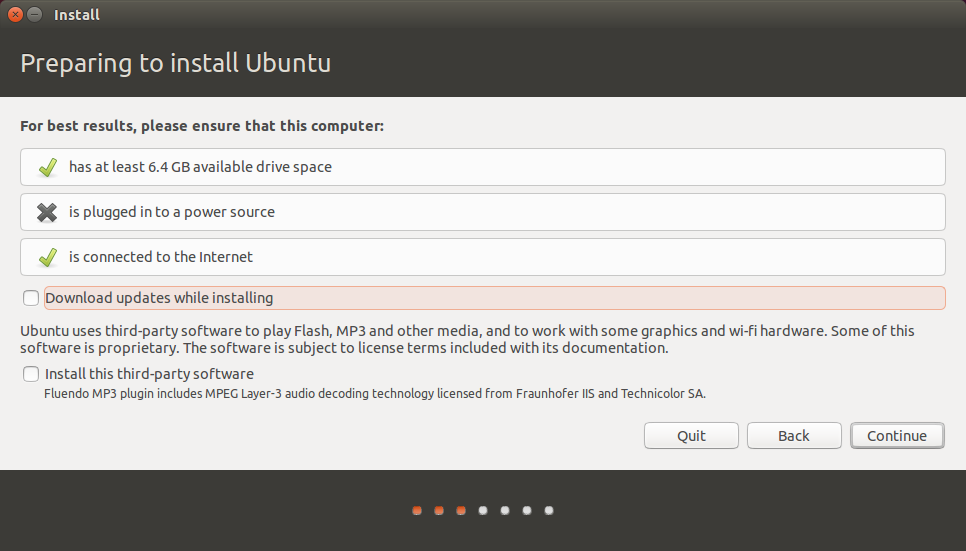
\includegraphics[scale=0.5]{pics/5.png}\\
\end{center}

در بخش بعد اوبونتو به شما چند انتخاب می‌دهد.
\begin{description}
\item[انتخاب اول]: نصب اوبونتو در کنار سیستم‌عامل فعلی\\
اگر دستگاه شما به اندازهٔ کافی (حداقل ۸ گیگابایت) فضای خالی داشته باشد، این 
گزینه برای شما نمایش داده می‌شود و اوبونتو به میزان دلخواه خودش، بخشی از فضای 
خالی روی هارد شما را به خودش اختصاص می دهد.

\item[انتخاب دوم]: پاک کردن سیستم‌عامل فعلی و نصب اوبونتو به جای آن\\
اگر دیگر تمایلی به استفاده از سیستم‌عامل فعلی خودتان ندارید، می‌توانید با انتخاب 
این گزینه اوبونتو را به جای آن جایگزین کنید. توجه داشته باشید که در صورت انتخاب 
این گزینه، تمام اطلاعات شما پاک خواهد شد.

\item[انتخاب سوم]: تنظیمات دستی (\lr{Something Else})\\
در این قسمت شما می‌توانید تنظیمات دلخواه خودتان را داشته باشید؛ مثلا یکی از 
پارتیشن‌های خود را پاک کرده و به اوبونتو اختصاص دهید.\\
\begin{center}
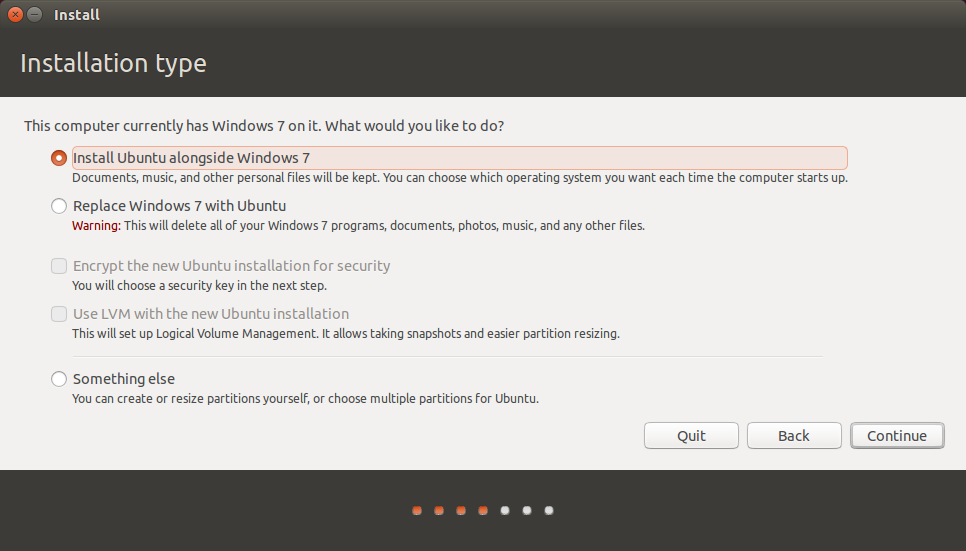
\includegraphics[scale=0.5]{pics/6.png}\\
\end{center}
* اگر فضای خالی ندارید و به پاک‌کردن یکی  از پارتیشن‌هایتان نیز متمایل نیستید، 
می‌توانید از فضای نصب خارج شده و در بخش امتحان زنده اوبونتو با برنامهٔ 
\lr{GParted} بخشی از فضای خالی پارتیشن  دلخواه خود را انتخاب کنید و آن را از 
پارتیشن جدا کنید و یا این‌که این کار را با برنامه‌های مخصوص کار با پارتیشن‌ها در 
سیستم‌عامل فعلی‌تان انجام دهید.
\end{description}

اوبونتو به حداقل ۲ پارتیشن احتیاج دارد: اولی پارتیشن اصلی و دیگری پارتیشنی برای 
حافظهٔ مجازی.\\
برای اضافه‌کردن حافظهٔ مجازی، شما باید روی \lr{+} (\lr{Add}) کلیک کنید و در بخش 
نوع پارتیشن (\lr{Type for the new partition}) گزینهٔ \lr{Logical} را انتخاب 
کنید. در بخش \lr{New partition size in megabytes} هم میزان فضایی تقریبا برابر با 
رم دستگاه یا کمی بیش‌تر را بدهید و در بخش \lr{Use as}، گزینهٔ \lr{swap area} را 
انتخاب کنید. \lr{OK} را بزنید.\\
برای اضافه‌کردن پارتیشن بعدی، روی فضای خالی باقی‌مانده کلیک کنید و \lr{+} 
(\lr{Add}) را بزنید. در بخش نوع پارتیشن \lr{Primary} و در بخش \lr{Use as}، 
ترجیحاً \lr{Ext4} را انتخاب کنید. در قسمت \lr{Mount point} هم گزینهٔ \lr{/} را 
برگزینید.\\
\begin{center}
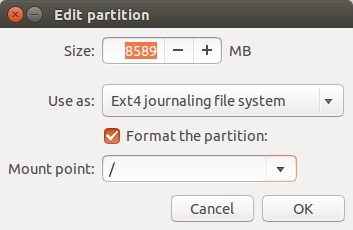
\includegraphics[scale=0.6]{pics/7.png}\\
\end{center}
پس از انجام این کارها، روی گزینهٔ \lr{Install Now} کلیک کنید تا اوبونتو شروع به 
نصب‌شدن کند.

\begin{center}
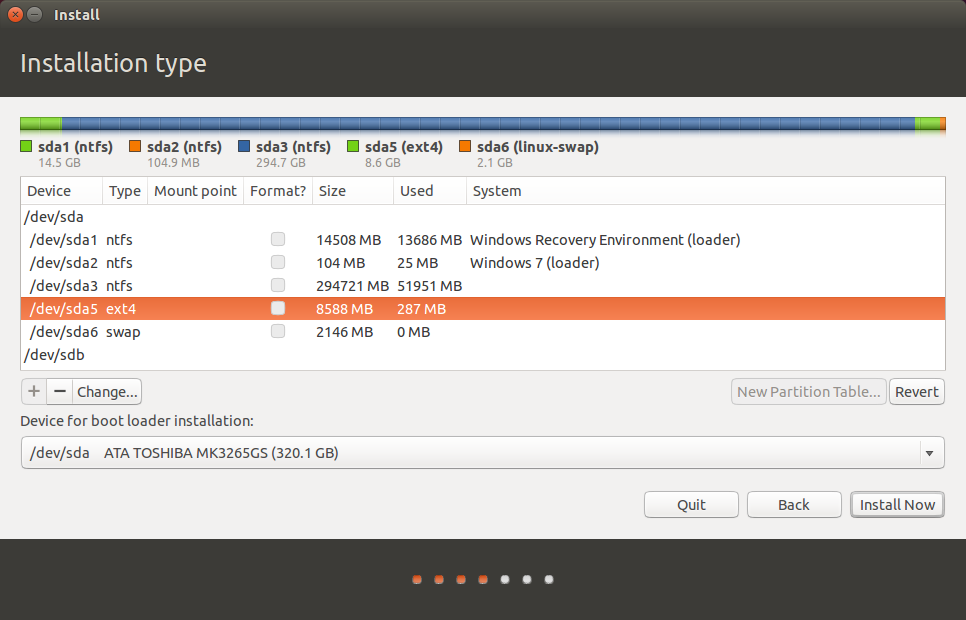
\includegraphics[scale=0.5]{pics/8.png}\\
\end{center}

در بخش بعد، روی محل زندگی خود در نقشه کلیک کنید تا زمان کامپیوتر را تنظیم 
کنید.\\
\begin{center}
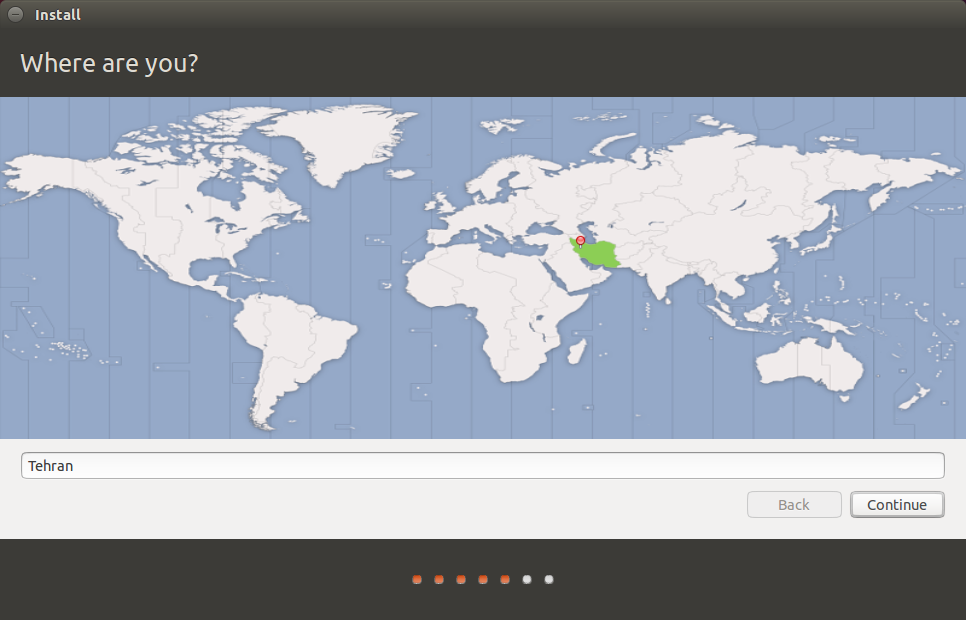
\includegraphics[scale=0.47]{pics/9.png}\\
\end{center}
در بخش بعد زبان \lr{Persian} را انتخاب کنید و روی ادامه (\lr{Continue}) کلیک 
کنید.

\begin{center}
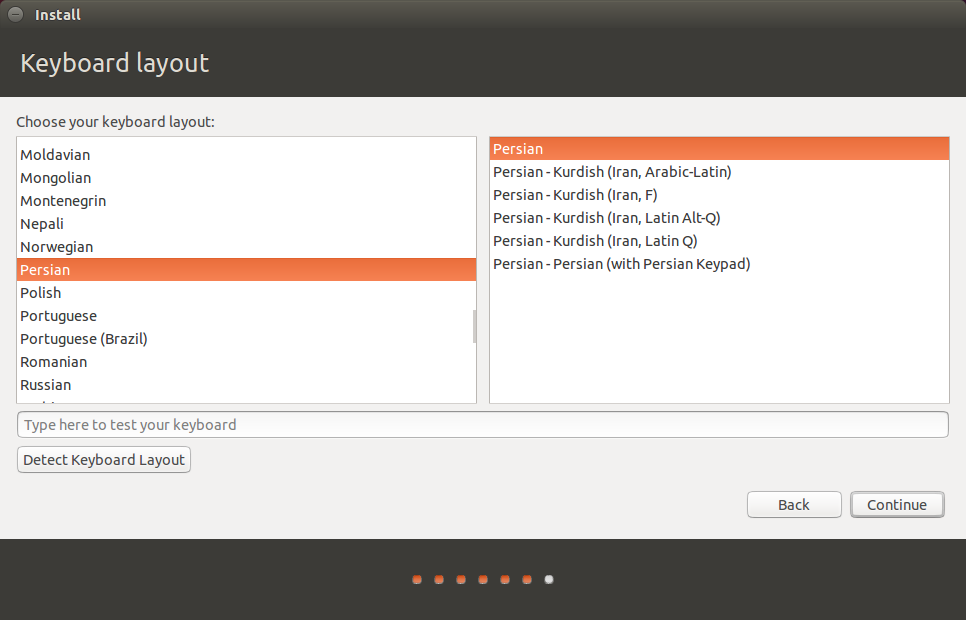
\includegraphics[scale=0.47]{pics/10.png}\\
\end{center}

در این قسمت مشخصات کاربری خود را به‌همراه گذرواژه وارد کنید.
\begin{center}
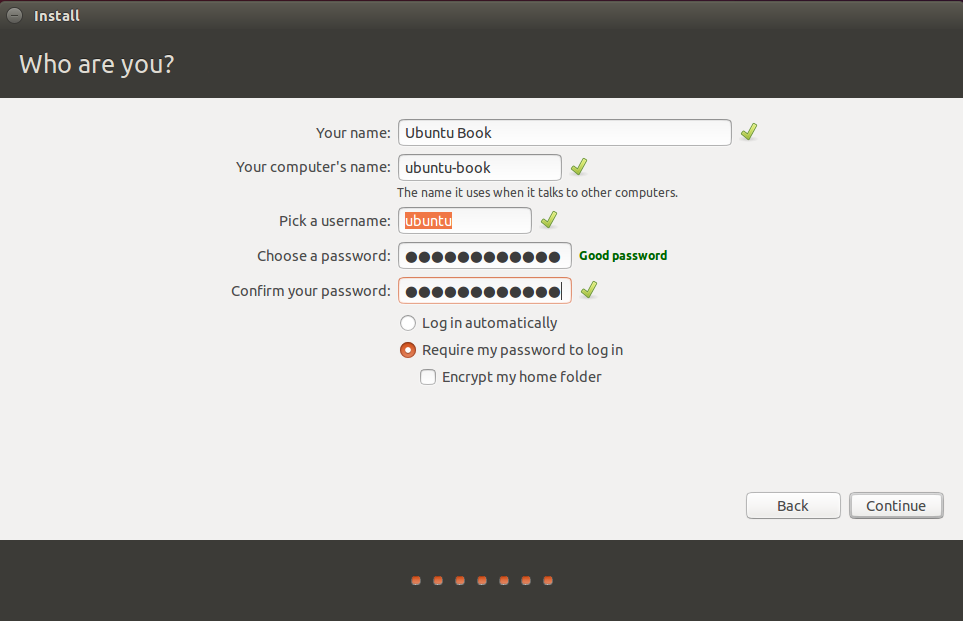
\includegraphics[scale=0.47]{pics/11.png}
\end{center}

اوبونتو خیلی سریع نصب خواهد شد. شما می‌توانید در این فرصت توضیحات مربوط به 
اوبونتو را مطالعه کنید تا نصب تمام شود.
\begin{center}
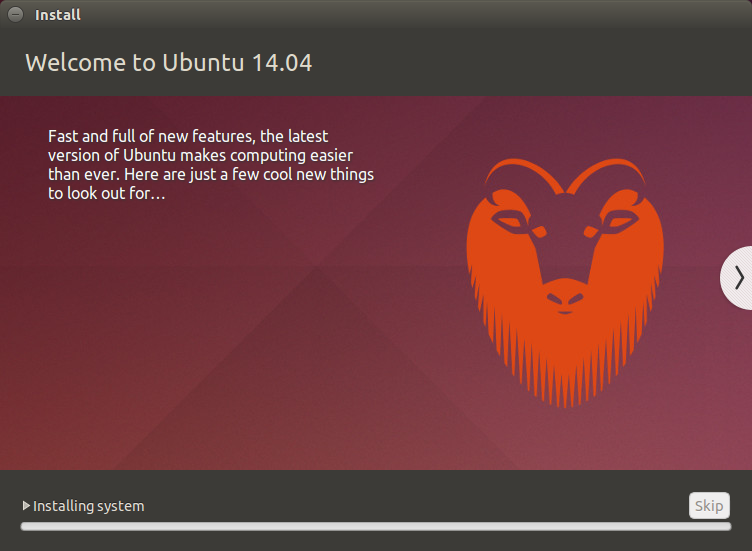
\includegraphics[scale=0.52]{pics/12.png}
\end{center}

\chapter{شروع کار با یونیتی}
حالا شما مراحل نصب را پشت سر گذاشته‌اید و اگر پا به پای این کتاب پیش رفته باشید، در صفحهٔ ورود اوبونتو قرار دارید.\\
\begin{center}
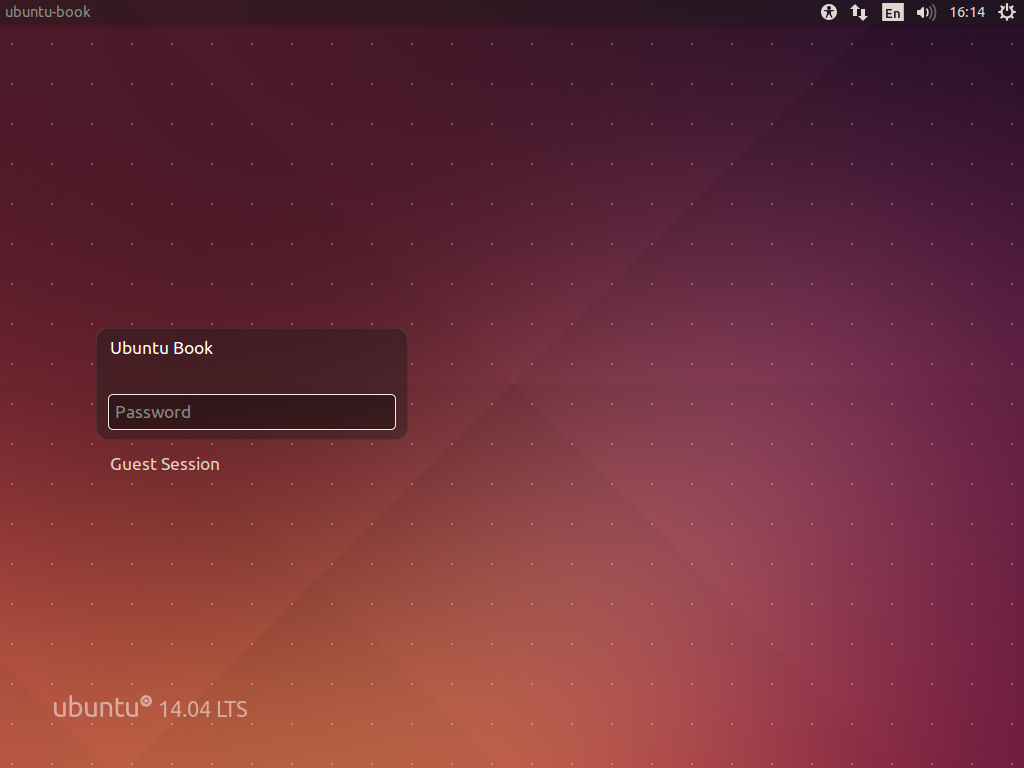
\includegraphics[scale=0.65]{pics/13.png}
\end{center}

بعد از واردکردن گذرواژه، وارد صفحهٔ زیر می‌شوید. این همان یونیتی است، محیطی که به طور پیش‌فرض در اوبونتو با آن کار خواهید کرد.
\begin{flushleft}
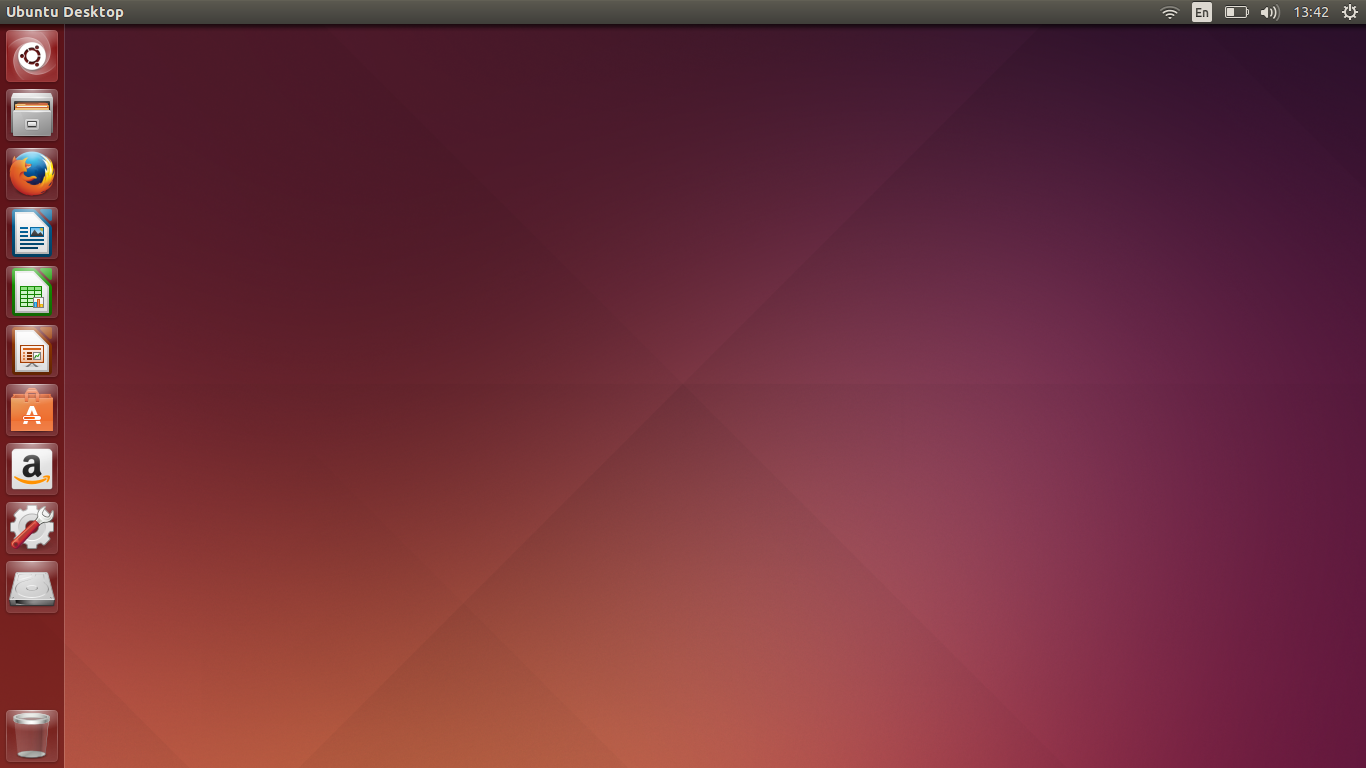
\includegraphics[scale=0.38]{pics/14.png}
\end{flushleft}

\section{یونیتی چیست؟}
یونیتی محیطی است که سادگی، زیبایی، قدرت و یکپارچگی را هم برای کاربران و هم برای توسعه‌دهندگان نرم‌افزار فراهم می‌کند.\\
هیچ جای نگرانی نیست؛ یونیتی تماماً ویژگی‌های محیط‌های قبلی را که با آن‌ها احتمالاً در ویندوز یا سیستم‌عامل اپل کار کرده‌اید دارد. ویژگی‌هایی مانند کشیدن و رهاکردن، کلیک‌کردن روی آیکون‌ها، قابلیت کپی‌کردن و بسیاری دیگر.
در ادامه بیش‌تر با یونیتی آشنا خواهید شد.
\subsection{تاریخچهٔ یونیتی}
شاید برای‌تان جالب باشد که یونیتی از کجا آمده است، چه گروهی آن را توسعه می‌دهند و از ابتدا روی اوبونتو بوده است یا نه.\\
یونیتی محیط کاری است که در حال حاضر تنها روی توزیع اوبونتو در دسترس است و توسط تیم اوبونتو در حال توسعه است. یونیتی یکی از جوان‌ترین محیط‌های کاری است. در‌واقع، یونیتی از توزیع ۱۱/۰۴ روی اوبونتو قرار گرفت و عمری حدود ۳ سال دارد؛ اما توانسته در همین مدت کوتاه محیطی بسیار ساده، زیبا و کارآمد را به کاربران خود ارائه دهد. یونیتی با هدفِ عرضهٔ اوبونتو روی دستگاه‌های دیگر (تبلت‌ها و گوشی‌ها و تلویزیون‌های هوشمند) و ظاهری یکپارچه برای تمامی دستگاه‌ها طراحی شده است و در هر نسخه به ویژگی‌ها و پایداری آن افزوده می‌شود. اوبونتوی ۱۴/۰۴ از نسخهٔ ۷/۲ یونیتی استفاده می‌کند.
\section{واسط کاربری یونیتی}
ظاهر یونیتی شامل بخش‌های زیر است:\\
\begin{itemize}
\item میزکار
\item اجراگر (\lr{Launcher})
\item پنل
\item داشبورد
\item هود
\end{itemize}

\subsection{میزکار}
محیط اصلی شماست. در این محیط شما می‌توانید برنامه‌ها و پنجره‌های مختلف را باز یا بسته کنید.
\subsection[اجراگر (Launcher)]{اجراگر (\lr{Launcher})}
اجراگر همان سکویی است که در سمت چپ به صورت عمودی قابل مشاهده است. در لانچر، تمام برنامه‌های باز شما نمایش داده می‌شود. همچنین شما می‌توانید برنامه‌هایی را که بیش‌تر به آن‌ها نیاز دارید، در آن‌جا نگه دارید تا با سرعت بیش‌تری به آن‌ها دسترسی داشته باشید.

\subsubsection{راهنمای اجراگر}
برای اضافه و حذف‌کردن آیکن یک برنامه به اجراگر، کافی است روی لوگوی اوبونتو کلیک کنید و نام یا ویژگی برنامهٔ مورد نظر خود را تایپ کنید و بعد آیکن آن برنامه را با موس گرفته و به روی اجراگر بکشید و رهایش کنید. برای حذف‌کردن نیز تنها کافی است روی آن آیکن کلیک راست موس را بزنید و روی \lr{Unlock from Launcher} کلیک کنید؛ یا این‌که آیکن را گرفته و آن را بر روی آیکن سطل زباله برده و رها کنید تا آیکن برنامه از اجراگر حذف شود.

\begin{center}
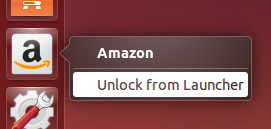
\includegraphics[scale=0.5]{pics/15.png}
\end{center}

\subsection{هود}
فرایند گشتن در منوهای تودرتو و پیچیده و به خاطر سپردن موقعیت زیرمنوها همیشه کاری بیهوده و زمانبر بوده است. یونیتی با \lr{Hud} به شما امکان جست‌و‌جوی سریع و بی‌دردسر را در منوها می‌دهد. با زدن کلید \lr{Alt} در پنجرهٔ برنامهٔ در حال اجرا، هود را فعال کرده و در منوهای آن پنجره جست‌وجو کنید.\\
\begin{center}
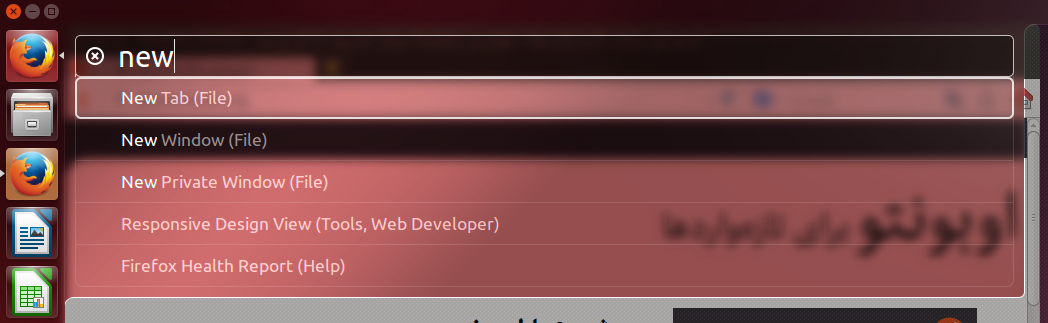
\includegraphics[scale=0.5]{pics/16.png}
\end{center}

\subsection{پنل}
پنل همان نواری است که در بالاترین قسمت از محیط خود آن را می‌بینید. در پنل، اطلاعاتی مانند منوی تنظیمات، ساعت و تاریخ ، صدا، شبکه و منوی من (که برای اطلاع از آخرین وضیعت پیام‌های پست الکترونیکی و شبکه‌های اجتماعی و چت با دوستان‌تان است) قابل مشاهده‌اند. اما شاید مهم‌ترین چیزی که در پنل به آن نیاز دارید، منوی پنجره‌ای است که در آن مشغول به کار هستید.

\subsubsection{ویژگی‌های پنل}
پنل از دو بخش تشکیل شده است: بخش سمت راست که در آن منوی تنظیمات، ساعت و تاریخ، تنظیمات صدا، تنظیمات شبکه، منوی من، نمایش باتری (در صورت استفاده از لپ‌تاپ) و تغییر زبان قرار گرفته و در سمت چپ، منوی برنامه وجود دارد که ابتدا نام پنجرهٔ فعال در آن نمایان است، اما با بردن موس بر روی سمت چپ پنل این منو نمایان می‌شود. این قابلیت یونیتی باعث می‌شود که وقتی به منو احتیاجی ندارید، از دید پنهان باشد.
\begin{flushleft}

\includegraphics[scale=0.39]{pics/17.png}
\end{flushleft}

\begin{description}
\item[منوی من] \hfill \\
در منوی من که به شکل یک پاکت نامه در بالا نمایان است، به موارد زیر دسترسی خواهید داشت:
\begin{itemize}
\item نوع وضعیت در برنامه‌های گفت‌وگو (چت)
\item دسترسی و مدیریت حساب‌های شبکه‌های اجتماعی
\item دسترسی و مدیریت پست الکترونیکی
\item دسترسی به برنامه‌های تحت وب نصب‌شدهٔ مرتبط
\end{itemize}

\begin{center}
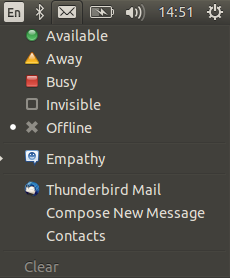
\includegraphics[scale=0.5]{pics/18.png}
\end{center}

این پاکت نامه، در صورتی که پیغامی خوانده‌نشده داشته باشید، به رنگ آبی در می‌آید. همچنین شما می‌توانید با کلیک وسط موس روی این پاکت نامه، به نشانه اطلاع‌تان از پیغام، رنگ‌اش را به رنگ اولیه تغییر دهید.


\item[نشانگر شبکه] \hfill \\
شما در این منو می‌توانید شبکهٔ بی‌سیم خود را انتخاب کنید و با واردکردن گذرواژه از این شبکهٔ بی‌سیم استفاده کنید. همچنین، این منو دسترسی سریع شما را به تنظیمات شبکه و \lr{VPN} فراهم می‌کند.
\begin{center}
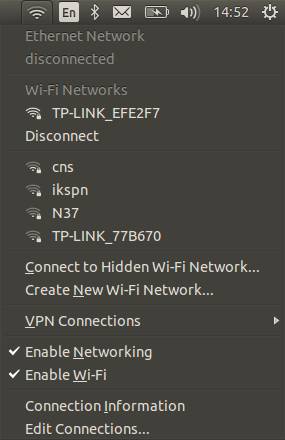
\includegraphics[scale=0.5]{pics/19.png}
\end{center}

\item[نشانگر صدا] \hfill \\
در این نشانگر قادر خواهید بود صدا را کم یا زیاد کنید. همچنین امکان پخش یا تغییر آهنگِ در حال پخش نیز وجود دارد.
\begin{center}
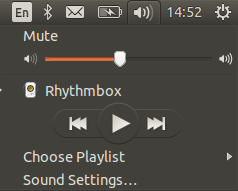
\includegraphics[scale=0.5]{pics/20.png}
\end{center}

\item[نشانگر ساعت] \hfill \\
در این نشانگر شما به تنظیمات ساعت، تاریخ و تقویم ماهانه دسترسی خواهید داشت.
\begin{center}
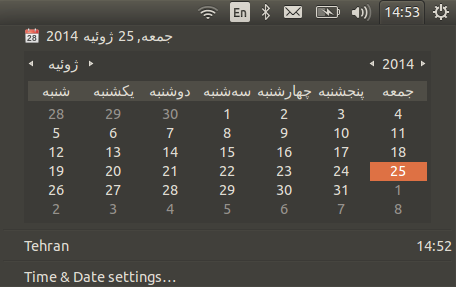
\includegraphics[scale=0.5]{pics/21.png}
\end{center}

\item[نشانگر تنظیمات] \hfill \\
در این بخش به تنظیمات سیستم، خاموش‌کردن یا شروع مجدد سیستم و سوییچ‌کردن از یک حساب کاربری به حساب کاربری دیگر دسترسی دارید.
\begin{center}
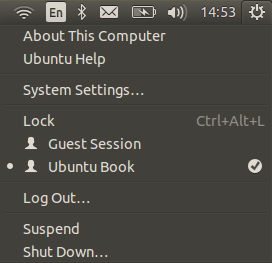
\includegraphics[scale=0.5]{pics/22.png}
\end{center}

\end{description}

\subsection{داشبورد}
داشبورد واسطی است که سریع‌ترین و راحت‌ترین راه دسترسی به فایل‌ها و برنامه‌ها را برای کاربران فراهم می‌کند. شما به کمک داشبورد می‌توانید نام برنامه یا کلمهٔ کلیدی آن را جست‌وجو کنید. همچنین می‌توانید برای جست‌وجوی خود محدودیت‌هایی را اعمال کنید تا فقط در آن دسته به دنبال نتیجه باشید. همچنین با بازشدن داشبورد به فایل‌ها و برنامه‌هایی که به تازگی استفاده کرده‌اید، دسترسی خواهید داشت.
\begin{center}
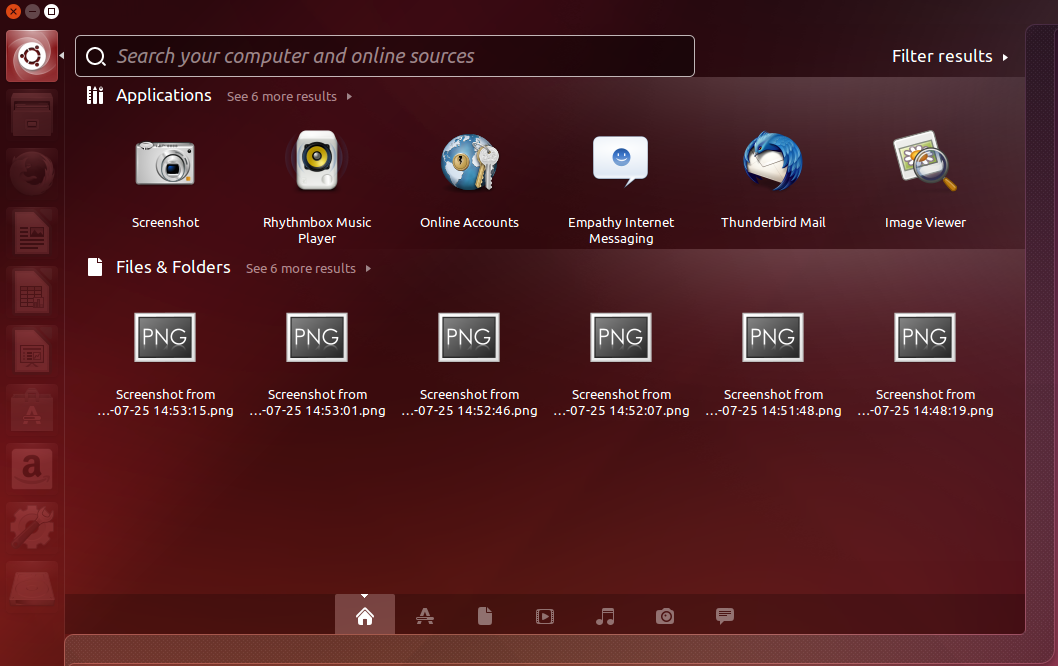
\includegraphics[scale=0.45]{pics/23.png}
\end{center}

\subsubsection{نحوهٔ دسترسی به داشبورد}
شما برای دسترسی به داشبورد، می‌توانید از ۲ راه استفاده کنید؛ راه اول این‌که می‌توانید با استفاده از موس روی بالاترین آیکون در لانچر (آیکون اوبونتو) کلیک کنید و داشبورد نمایان خواهد شد. همچنین می‌توانید در کیبورد دکمهٔ ویژه (که دکمهٔ ویندوز هم نامیده می‌شود) را فشار دهید تا داشبورد نمایان شود.

\subsubsection{ظاهر داشبورد}
داشبورد از بخش‌های زیر تشکیل شده است:
\begin{itemize}
\item جست‌وجو
\item نمایشگر
\item فیلتر
\item \textbf{لنزها}\\
دش به طور پیش فرض ۷ لنز دارد که هر لنز، برای دسترسی سریع‌تر شما به هدف‌تان طراحی شده است. این ۷ لنز عبارت‌اند از: لنز خانه که امکان دسترسی به آخرین فایل‌ها و برنامه‌ها را دارد، لنز برنامه‌ها که تنها برای نرم‌افزارهاست، لنز فایل‌ها که تنها بین فایل‌های شما جست‌وجو می کند، لنز فیلم که بین فیلم‌هایی که روی دستگاه شما قرار دارد و فیلم‌هایی که با آن موضوع در فضای اینترنت قرار دارد، جست‌وجو را انجام می‌دهد، لنز موسیقی که فایل‌های موسیقی موردنظر شما را روی کامپیوترتان و اینترنت پیدا می‌کند، لنز عکس بین عکس‌های شما می گردد و همین‌طور لنز اخیراً اضافه‌شدهٔ دوستان که به دنبال عبارات موردنظر شما در اکانت‌های شبکه‌های اجتماعی شما می‌گردد.
\begin{center}

\includegraphics[scale=0.65]{pics/24.png}
\end{center}

\end{itemize}

\subsubsection{پیش‌نمایش}
امکان مشاهدهٔ پیش‌نمایشی از محتواهای مختلف با کلیک راست روی آن در داشبورد وجود دارد. مثلا با کلیک راست روی آیکن \lr{Firefox} در داشبورد، توضیحاتی از آن به همراه اسکرین‌شات و امتیاز کسب‌شده از کاربران نشان داده می‌شود.

\begin{center}
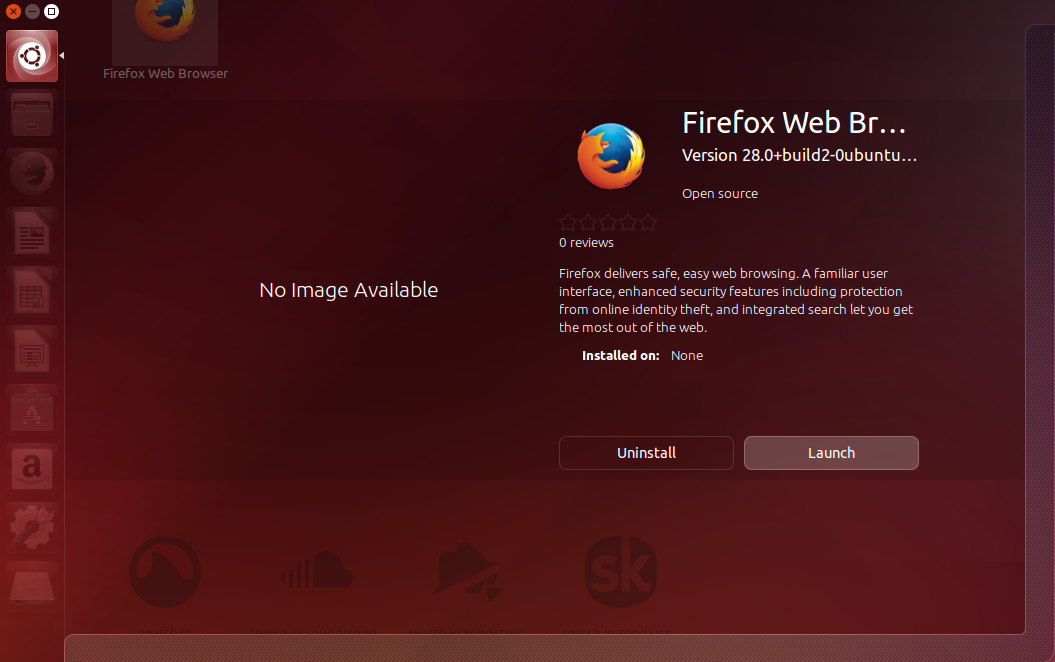
\includegraphics[scale=0.45]{pics/25.png}
\end{center}

پیش‌نمایش از برنامه‌ها، تصاویر، ویدیو، موزیک و تعدادی دیگر از قالب‌ها پشتیبانی می‌کند.

\begin{center}
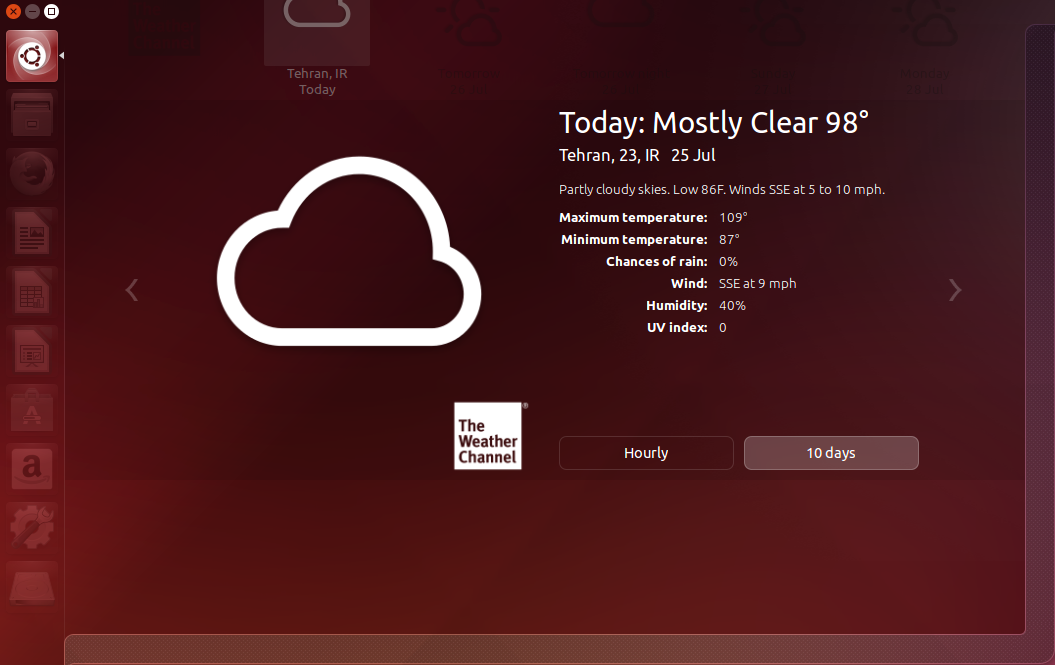
\includegraphics[scale=0.45]{pics/26.png}
\end{center}

\subsection{برنامه‌های تحت وب}
با کمک برنامه‌های تحت وب یا \lr{WebApps}، می‌توان وب‌سایت‌هایی مانند \lr{Gmail}، \lr{Grooveshark}، \lr{Last.fm}، \lr{Facebook} و بسیاری دیگر را با محیط \lr{Unity} یکپارچه کرد. برای مثال، با نصب \lr{WebApp}های مناسب، می‌توانید \lr{Grooveshark} را با منوی صدا کنترل و پیام‌های جدید \lr{Google+}‎ را با سیستم اعلان اوبونتو دریافت نمایید. \lr{WebApp} \lr{Amazon} به صورت پیش‌فرض فعال است. \lr{WebApp} های بیش‌تر از مرکز نرم‌افزاری قابل نصب هستند؛ اما راه راحت‌تر آن است که با مرورگر \lr{Firefox}، سایت مورد نظر خود، مانند \lr{Gmail}، را باز کنید که بعد از آن پیشنهاد نصب (در صورت موجود بودن برنامه برای آن وب‌سایت) به شما داده می‌شود.

\begin{center}
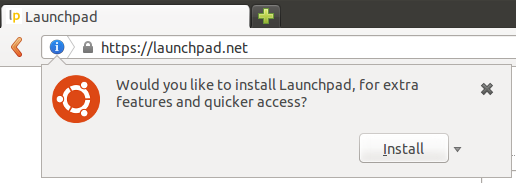
\includegraphics[scale=0.6]{pics/27.png}
\end{center}

\chapter{کارهای بعد از نصب}
\section{بررسی نکات انتشار}
 اوبونتو در هر نسخه پیشرفت‌های بسیاری می‌کند. آیا با پیشرفت‌های اوبونتوی ۱۴/۰۴ آشنا هستید؟ همین الان \href{https://wiki.ubuntu.com/TrustyTahr/ReleaseNotes}{نکات انتشار اوبونتو} را مطالعه کنید.


\section{نصب درایورها}
اگر از یک کاربر ویندوز بپرسید بعد از نصب ویندوز نوبت چیست، بدون شک جواب خواهد داد: «نصب درایور»! اکثر کاربرانی که از ویندوز به سمت اوبونتو کشیده می‌شوند، در اوایل به فکر دانلود و نصب درایورها هستند.\\
در اوبونتو عمدتاً نیاز به نصب درایور خارجی ندارید و این سیستم‌عامل بیش‌تر درایورهای مورد نیاز را به همراه دارد. اوبونتو را به صورت زنده بوت کنید و اگر همه چیز کار می‌کرد (صدا داشتید و صفحات وب را به خوبی توانستید مرور کنید)، آن را نصب کنید.\\
فقط ممکن است این احتمال وجود داشته باشد که اوبونتو بعضی از سخت‌افزارها، مثل کارت شبکه بی‌سیم را شناسایی نکند یا برای کارایی بیش‌تر گرافیکی، نیاز به نصب درایورهای انحصاری باشد.\\
برای نصب این درایورها، از \lr{System Settings}، گزینهٔ \lr{Software \& Updates} را انتخاب کنید و روی تب \lr{Additional Drivers} کلیک کنید. این ابزار سعی می‌کند برای سخت‌افزارهایی که شناخته نشده‌اند یا درایور بهتری برای‌شان موجود است، از اینترنت درایور را دانلود و سپس نصب کند.

\begin{center}
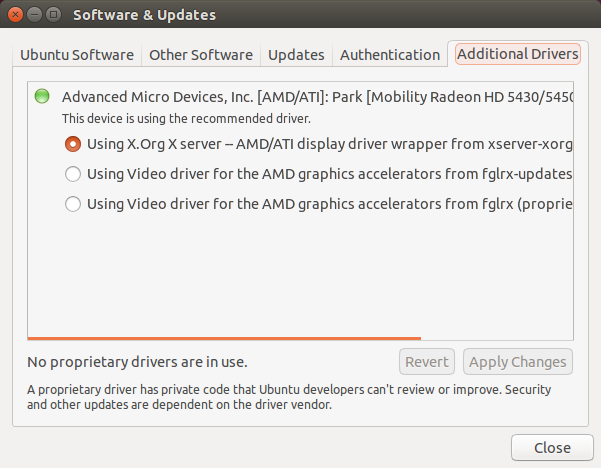
\includegraphics[scale=0.5]{pics/28.png}
\end{center}

\section{به‌روزرسانی لیست نرم‌افزارهای مخازن نرم‌افزاری}
در اوبونتو، برخلاف ویندوز، همهٔ نرم‌افزارهای موردنیاز را می‌توان از مخازن رسمی اوبونتو دانلود کرد. برای این‌که گنو/لینوکس‌تان از آخرین نسخهٔ نرم‌افزارها مطلع شود، لازم است لیست نرم‌افزارهای مخازن را به‌روز کنید. برای این کار، به اینترنت وصل شوید و برنامهٔ \lr{Terminal} را باز کنید و عبارت \lr{\texttt{sudo apt-get update}} را در آن تایپ کنید و کلید \lr{Enter} را بزنید. گذرواژه‌ٔ‌تان را وارد کنید (گذرواژه برای امنیت بیش‌تر، نشان داده نمی‌شود).

\begin{center}
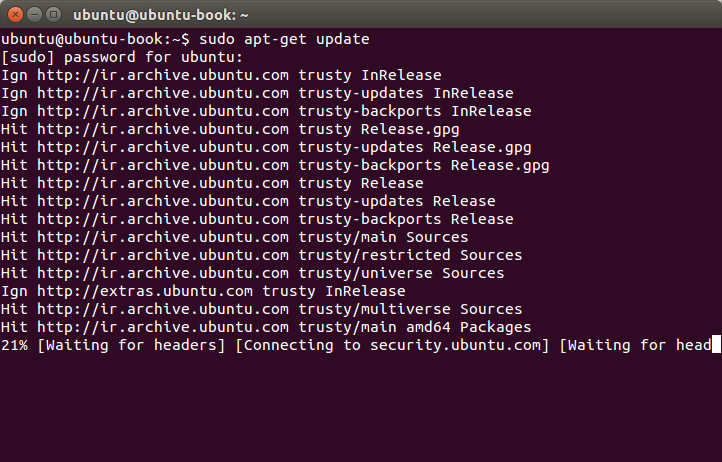
\includegraphics[scale=0.5]{pics/29.png}
\end{center}

\section[نصب کدک‌های چند رسانه‌ای، Flash Adobe و فونت‌های مناسب فارسی]{نصب کدک‌های چند رسانه‌ای، \lr{Adobe Flash} و فونت‌های مناسب فارسی}
اوبونتو بسیاری از کدک‌های صوتی و تصویری معروف مثل \lr{MP3}، فلش و \ldots  را به همراه ندارد. برای نصب آن‌ها، در مرکز نرم‌افزار (\lr{Software Center}) دنبال \lr{ubuntu-restricted-extras} بگردید و این بسته را نصب کنید.

\begin{center}
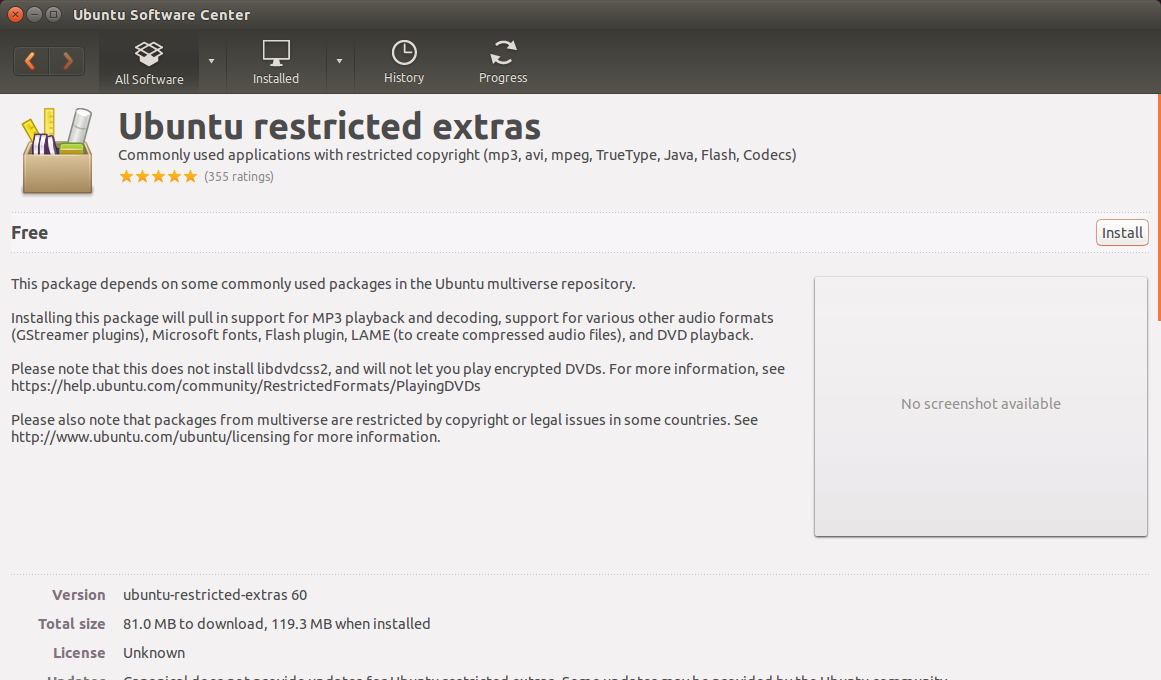
\includegraphics[scale=0.4]{pics/30.png}
\end{center}

\section{نصب برنامه‌های اضافی}
برنامه‌های همراه اوبونتو زیاد هستند، اما برای تمامی کارهای روزانه کفایت نمی‌کنند. صدها برنامهٔ آزاد و غیر آزاد وجود دارد که به راحتی یک کلیک از مرکز نرم‌افزار نصب می‌شوند. لیست زیر چند برنامهٔ پیشنهادی را معرفی می‌کند.
\begin{itemize}
\item \lr{Chromium}: مرورگر سریع کرومیوم
\item \lr{Gimp}: ابزاری قوی برای ویرایش و ساخت تصاویر پیکلسی، معادل \lr{Adobe Photoshop}
\item \lr{LibreCAD}: ابزار طراحی نقشه‌های ساختمانی، معادل \lr{AutoCAD}
\item \lr{GNU Octave}: ابزاری عالی برای رایانش عددی و تجسم داده، معادلی برای \lr{MATLAB}
\end{itemize}

\section{فعال‌کردن راست به چپ در لیبره‌آفیس}
برای این کار به این مسیر بروید:\\

\begin{center}
\lr{Langauges} \textsf{→} \lr{Language Settings} \textsf{→} \lr{Options} \textsf{→} \lr{Tools}\\
\end{center}

تیک گزینه \lr{Complex text layout (CTL)} را بزنید و سپس \lr{Persian} را از لیستی که فعال می‌شود، برگزینید.

\begin{center}
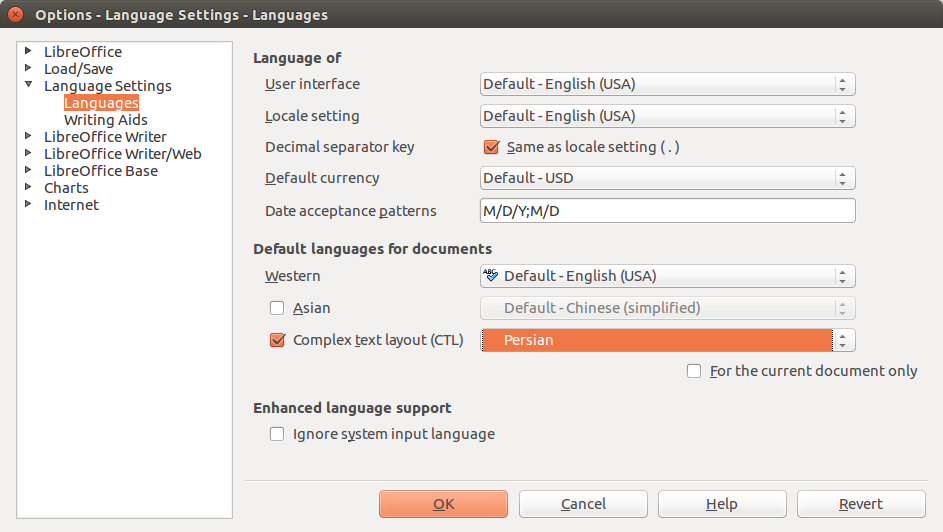
\includegraphics[scale=0.55]{pics/31.png}
\end{center}

\section{استفاده از میزکار متفاوت}
اوبونتو به همراه میزکار \lr{Unity} عرضه می‌شود، ولی آن را به شما تحمیل نمی‌کند. برای داشتن میزکار \lr{KDE}، بستهٔ \lr{kubuntu-desktop} و برای داشتن \lr{Gnome Shell}، بستهٔ \lr{gnome-shell} را نصب کنید.

\begin{center}
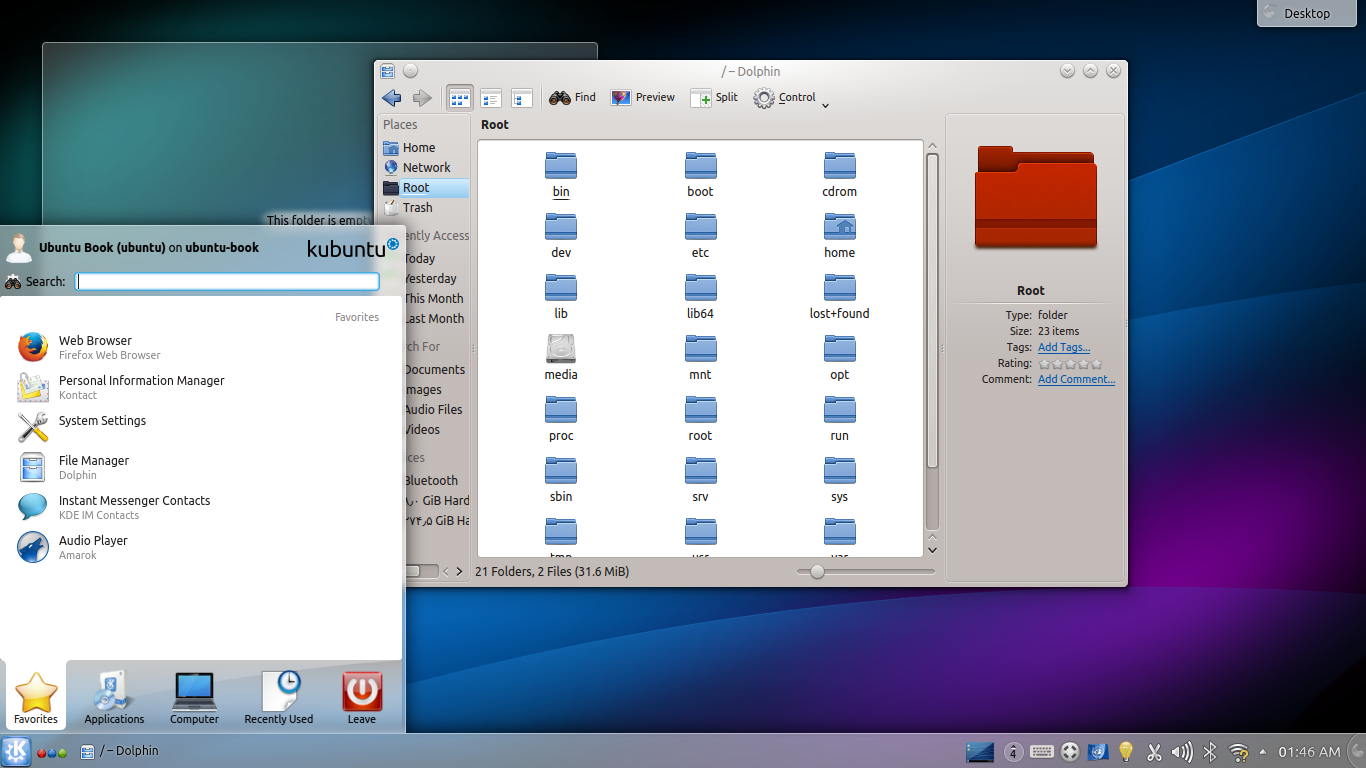
\includegraphics[scale=0.45]{pics/32.png}\\
نمایی از \lr{KDE}\\
\end{center}

\begin{center}
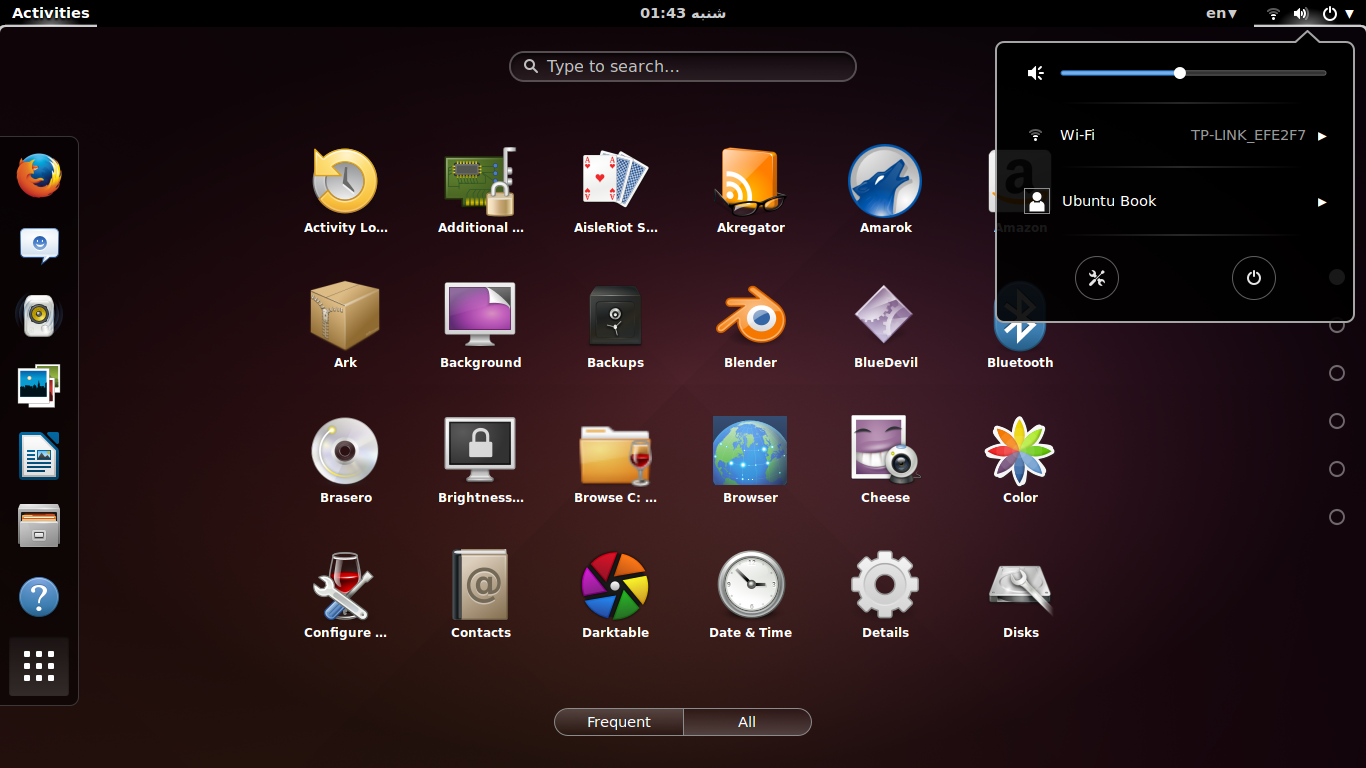
\includegraphics[scale=0.33]{pics/33.png}\\
نمایی از \lr{Gnome Shell}
\end{center}

\section{سفارشی‌سازی میزکار}
جدا از این‌که چه میزکاری استفاده می‌کنید، می‌شود آن را با مجموعهٔ آیکن، فونت و پوسته‌های مختلف شخصی‌سازی کرد. مجموعه‌ای از بهترین آیکن و پوسته‌ها را از \lr{gnome-look.org} و \lr{kde-look.org} بگیرید. راهنمای استفاده هم همان جا وجود دارد.
\begin{center}
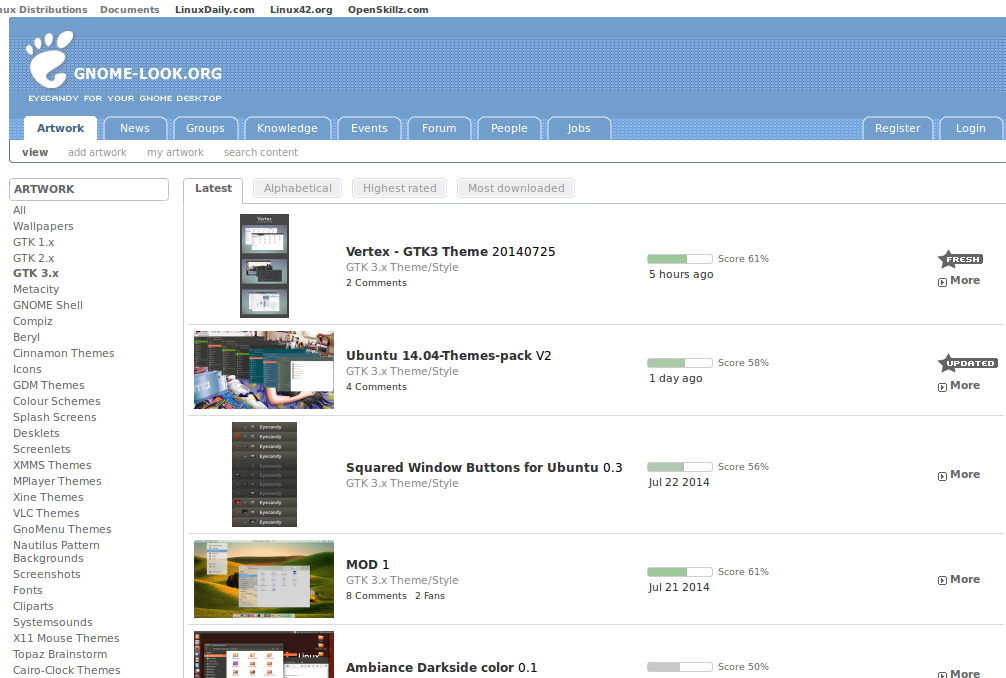
\includegraphics[scale=0.4]{pics/34.png}
\end{center}

\section{راه‌اندازی کلاینت ایمیل}
اوبونتو \lr{Thunderbird} را به همراه دارد که ابزاری برای مدیریت ایمیل‌هاست. بعد از اجرای تاندربرد، اسم، آدرس ایمیل و پسورد حساب ایمیل‌تان را به آن بدهید تا ایمیل‌هایتان را دریافت کند.

\section{همکاری در جامعهٔ کاربری اوبونتو}
اوبونتو با همکاری جامعهٔ کاربری‌اش زنده است و کتابی هم که می‌خوانید، با همکاری همین جامعهٔ کاربری ساخته شده است. تا جای ممکن، جامعهٔ کاربری را فراموش نکنید و به آن کمک کنید. \href{http://www.ubuntu.ir}{وب‌سایت فارسی اوبونتو} جای خوبی برای شروع است. تعداد بسیار زیادی سوال در انجمن بدون پاسخ مانده‌اند و ده‌ها مدخل در ویکی وجود دارد که نیازمند به‌روزرسانی است.

\section{معرفی اوبونتو به دوستان و آشنایان}
اوبونتو را به دوستان و همکاران‌تان معرفی کنید تا آن‌ها هم با این سیستم‌عامل فوق‌العاده و آزاد آشنا بشوند.

\chapter{نصب نرم‌افزار در اوبونتو}
در این فصل به نحوهٔ نصب نرم‌افزار، یکی از مهم‌ترین کارهایی که در هر سیستم‌عامل به طور معمول انجام می‌دهیم، می‌پردازیم. برای نصب نرم‌افزار در اوبونتو دو راه وجود دارد: استفاده از رابط گرافیکی تقریباً جدید اوبونتو به نام \lr{Ubuntu Software Center} و استفاده از \lr{Apt} و رابط خط فرمان. البته نرم‌افزاری به نام \lr{Synaptic} هم وجود دارد که یک رابط گرافیکی برای \lr{Apt} ارائه می‌دهد و در همین فصل به معرفی آن می‌پردازیم.

\section[آشنایی با Center Software Ubuntu]{آشنایی با \lr{Ubuntu Software Center}}
مرکز نرم‌افزاری اوبونتو از نسخهٔ ۹/۱۰ به اوبونتو اضافه شد و هدف آن ساده‌تر شدن نصب برنامه در اوبونتو بود. تا قبل از ارائهٔ \lr{Ubuntu Software Center}، نصب نرم‌افزار در اوبونتو تنها از راه دستورات \lr{Apt} و \lr{Synaptic} ممکن بود و به همین دلیل، کاربران تازه‌کار با مشکلات زیادی روبه‌رو بودند. مرکز نرم‌افزاری اوبونتو رابط زیبایی دارد و شبیه بیش‌تر \lr{Sofware Center}های کنونی است.

\subsection[محیط Center Software Ubuntu]{محیط \lr{Ubuntu Software Center}}
آیکن \lr{Software Center} به صورت پیش‌فرض در اجراگر قرار دارد. اگر هم آن را حذف کرده‌اید، آن را جست‌وجو و اجرا کنید. پنجرهٔ اصلی مرکز نرم‌افزاری اوبونتو باز می‌شود.

\begin{center}
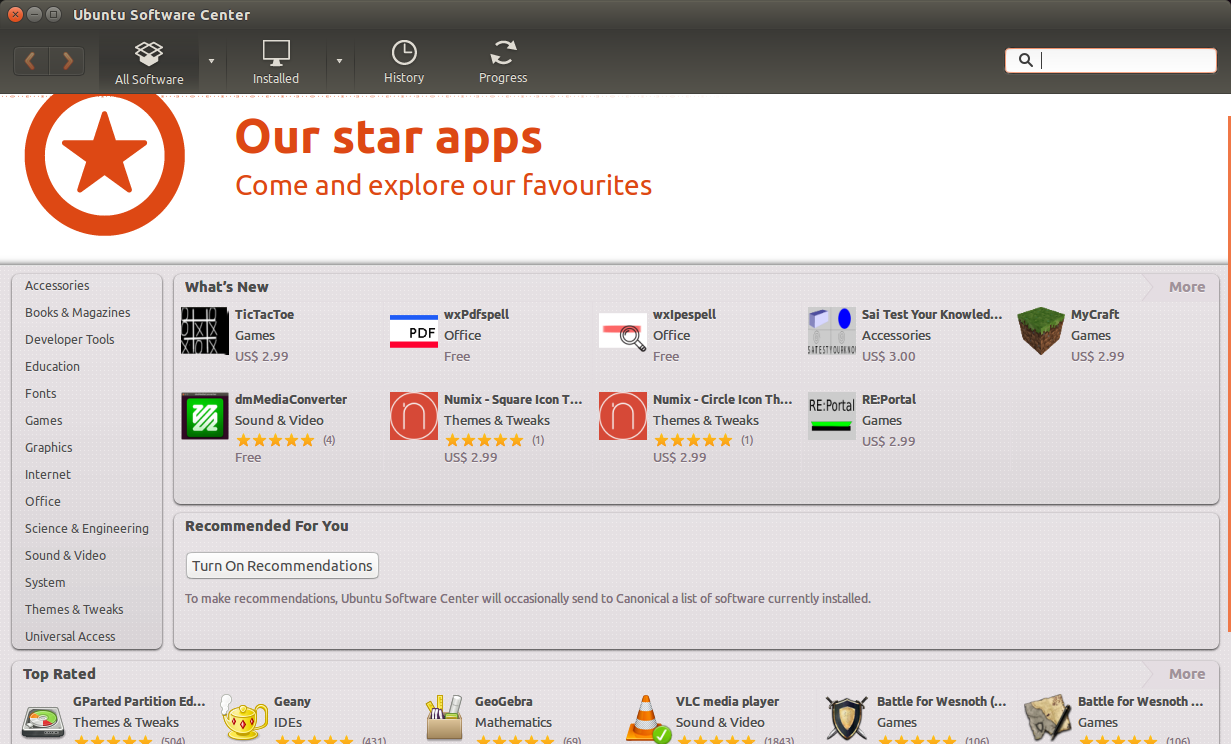
\includegraphics[scale=0.4]{pics/35.png}
\end{center}

این پنجره از بخش‌های مختلفی تشکیل شده است. در نوار بالایی، دکمه‌های جلورفتن و عقب‌رفتن، \lr{All Software} برای مشاهدهٔ همهٔ نرم‌افزارها، \lr{Installed} برای دیدن نرم‌افزارهای نصب‌شده، \lr{History} برای دیدن سوابق حذف و نصب نرم‌افزار، \lr{Progress} برای آگاهی از وضعیت دانلود و نصب نرم‌افزارهایی که دستور نصب‌شان را داده‌اید و کادر جست‌وجو وجود دارد. \lr{All Software} و \lr{Installed} دارای منوی بازشونده هستند که می‌توانید با انتخاب گزینه‌های آن نرم‌افزارهای یک مخزن مشخص را ببینید. \lr{USC} به صورت پیش‌فرض روی گزینهٔ \lr{All Software} قرار دارد.\\
در بخش اصلی، درست زیر نوار بالایی، \textbf{بنر نمایشی} وجود دارد که دارای حالتی تبلیغاتی است و نرم‌افزارهایی را به شما معرفی می‌کند. زیر بنر، بخش \textbf{نرم‌افزارهای تازه} وجود دارد و در پایین آن نیز بخش \textbf{نرم‌افزارهای پیشنهادی} را می‌بینید که البته باید آن را فعال کنید. در پایین صفحه هم برنامه‌هایی معرفی می‌شوند که بالاترین امتیاز را از کاربران دریافت کرده‌اند. در سمت چپ نیز لیست دسته‌بندی‌شدهٔ نرم‌افزارها وجود دارد که با کلیک روی هر یک از گزینه‌های آن می‌توانید نرم‌افزارهای همان بخش را مشاهده کنید.\\
نصب نرم‌افزار در \lr{USC} بسیار ساده است. تنها کافی است که نرم‌افزار مورد نظر خود را پیدا کنید و در صفحهٔ آن نرم‌افزار روی \lr{Install} کلیک کنید. گذرواژهٔ سیستم از شما پرسیده می‌شود و بعد از دانلودشدن فایل‌های مورد نیاز، برنامه نصب خواهد شد.

\section[آشنایی با Apt]{آشنایی با \lr{Apt}}
\lr{Apt} (مخفف \lr{Advanced Packaging Tool})، برنامهٔ نصب و حذف نرم‌افزارها در توزیع دبیان گنو/لینوکس است. از آن‌جایی که اوبونتو از دبیان مشتق شده است، اوبونتو نیز \lr{Apt} را به همراه دارد. نرم‌افزارهایی مثل \lr{Ubuntu Software Center} و \lr{Synaptic} هم تنها رابطی گرافیکی برای \lr{Apt} اند. پس آشنایی با \lr{Apt} می‌تواند در کنترل بیش‌تر بر سیستم به ما کمک کند.

\subsection{لیست مخازن}
برای این که \lr{Apt} کار کند، به لیست مخازن نیاز دارد. لیست مخازن شامل آدرس مکان‌هایی است که می‌توان از آن‌جا برای اوبونتو نرم‌افزار تهیه کرد. یکی از تفاوت‌های اصلی ویندوز و گنو/لینوکس نیز همین است. در اوبونتو به احتمال خیلی زیاد به هیچ‌گونه \lr{CD} و \lr{DVD}ای برای نصب نرم‌افزارها نیاز نخواهید داشت. حتا اغلب اوقات هم لازم نیست برای نصب یک نرم‌افزار به دنبال فایل نصب‌اش در اینترنت بگردید. بیش‌تر نرم‌افزارهای مورد نیاز در مخازن رسمی اوبونتو موجودند.\\
مخازن رسمی اوبونتو روی اینترنت‌اند. هرچند تمام نرم‌افزارهای مخازن اوبونتو بر روی چند \lr{DVD} هم قابل تهیه است، اما باید توجه داشت که نرم‌افزارهای مخازن همیشه در حال به‌روزآوری‌اند. پس برای استفاده از جدیدترین نسخه‌های نرم‌افزارها به اینترنت نیازمندید. البته حجم نرم‌افزارهای اوبونتو (و کلاً گنو/لینوکس‌ها)، به مراتب از ویندوز کم‌تر است. دلیل این موضوع، استفاده‌کردن نرم‌افزارهای گنو/لینوکسی از ابزارها و کتاب‌خانه‌های مشترک است.\\
\subsubsection{محل لیست مخازن}
لیست مخازن در گنو/لینوکس‌های بر پایهٔ دبیان (شامل اوبونتو)، یک فایل متنی به نام \lr{sources.list} است که در مسیر \lr{\texttt{/etc/apt/sources.list}} قرار دارد. برای ویرایش این فایل، باید فایل را در ویرایشگرهای متن باز کنید. در اوبونتو، دو ویرایشگر \lr{gedit} و \lr{Nano} وجود دارد که به ترتیب گرافیکی و متنی‌اند. کار با \lr{gedit} بسیار راحت‌تر از \lr{Nano} است، پس فایل را با \lr{gedit} باز می‌کنیم. اما ویرایش‌کردن فایل لیست مخازن نیازمند اجازهٔ ریشه است؛ در نتیجه، راحت‌ترین راه بازکردن این فایل با مجوز ریشه، استفاده از دستور \lr{\texttt{sudo gedit /etc/apt/sources.list}} است.\\
بعد از زدن دستور، پنجره‌ای مانند پنجرهٔ زیر باز می‌شود.\\
تعدادی خط را می‌بینید. اگر خطی در ابتدایش علامت \lr{\texttt{\#}} وجود داشته باشد، غیرفعال است. بقیه فعال‌اند و \lr{Apt} آن‌ها را می‌خواند.

\begin{center}
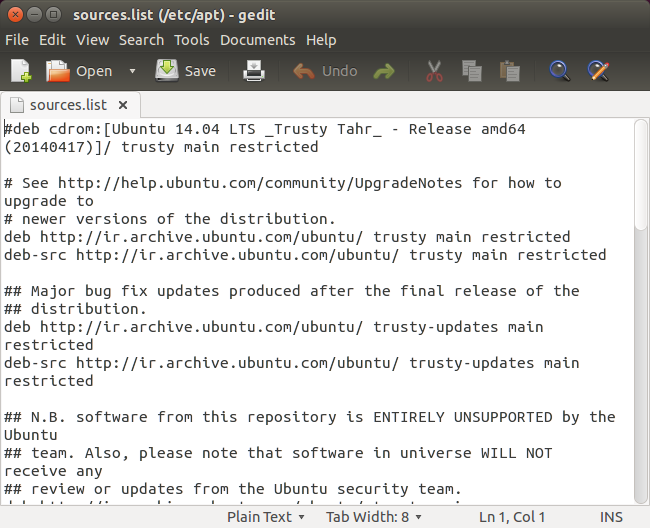
\includegraphics[scale=0.5]{pics/36.png}
\end{center}

\subsubsection{مفهوم خطوط لیست مخازن}
هر خط در این فایل شامل ۴ بخش به شکل \lr{\texttt{deb address distro component1 component2}} است. بخش اول، یعنی «\lr{\texttt{deb}}»، مشخص می‌کند که آرشیو مورد نظر دارای فایل‌های نصب با پسوند \lr{deb} است. در این بخش، به جای «\lr{\texttt{deb}}»، «\lr{\texttt{deb-src}}» هم می‌تواند قرار بگیرد که یعنی آرشیو دارای فایل‌های منبع است، نه فایل‌های نصب دبیانی.\\
در بخش دوم یا «\lr{\texttt{address}}»، باید آدرس مخزن را وارد کنید که می‌تواند آدرسی اینترنتی یا آدرسی محلی و روی کامپیوتر یا شبکهٔ خانگی‌تان باشد، اما اکثراً این یک آدرس اینترنتی است.\\
در بخش «\lr{\texttt{distro}}»، نام توزیع کنونی‌تان را وارد کنید. مثلاً برای اوبونتوی ۱۴/۰۴، باید «\lr{\texttt{trusty}} نوشته شود.\\
در آخرین قسمت هم نوع مخزن را وارد می‌کنید. اوبونتو مخازن مختلفی به نام‌های «\lr{main}»، «\lr{universe}»، «\lr{multiverse}»، «\lr{restricted}» و \ldots دارد.\\
در بخش آخر، می‌توان چندین نوع مخزن را وارد کرد. یعنی بعد از قسمت سوم، هر چه که وارد شود، مربوط به نوع مخزن خواهد بود.

\subsection[دستورهای معمول و اصلی Apt]{دستورهای معمول و اصلی \lr{Apt}}
\lr{Apt} نام یک ابزار است و اصولاً دستوری به شکل \lr{\texttt{apt}} وجود ندارد. برای استفاده از ابزار \lr{Apt}، باید از دستورهای زیرمجموعهٔ آن، مثل \lr{\texttt{apt-get}} و \lr{\texttt{apt-cache}} استفاده کرد. دستور \lr{\texttt{apt-get}}، بیش‌ترین استفاده را برای ما دارد.

\subsubsection[apt-get]{\lr{apt-get}}
همان‌گونه که گفته شد، دستور \lr{\texttt{apt-get}} مهم‌ترین دستور است. چون این دستور در بعضی فایل‌ها و پوشه‌های اصلی سیستم تغییر ایجاد می‌کند، برای استفاده از آن، باید کاربر ریشه بود (یعنی باید با \lr{\texttt{sudo}} همراه شود).\\
از این دستور برای کارهای زیر استفاده می‌شود:

\begin{description}
\item [به‌روزآوری لیست نرم‌افزارهای مخازن]: با به کار بردن دستور \lr{\texttt{sudo apt-get update}}
\item [نصب نرم‌افزار]: با دستور \lr{\texttt{sudo apt-get install software}} که به جای \lr{\texttt{software}}، باید نام نرم‌افزار مورد نظر خود را بنویسید. اگر حجم فایل‌هایی که قرار است دانلود شود زیاد باشد، پیامی مبنی بر تأیید دانلود و نصب نرم‌افزار ظاهر می‌شود که با زدن دکمهٔ \lr{Enter} تأیید می‌شود.\\
از این دستور برای نصب نسخهٔ جدید نرم‌افزار هم می‌توان استفاده کرد.
\item [حذف نرم‌افزار]: با دستور \lr{\texttt{sudo apt-get remove software}} نرم‌افزار حذف می‌شود، اما فایل‌های پیکربندی آن روی سیستم باقی می‌ماند. برای حذف نرم‌افزار همراه با حذف فایل‌های پیکربندی آن، از دستور \lr{\texttt{sudo apt-get purge software}} استفاده کنید.
\item [آپدیت‌کردن همهٔ نرم‌افزارها]: برای این کار از دستور \lr{\texttt{sudo apt-get upgrade}} استفاده کنید.
\item [آپگرید به نسخهٔ جدید اوبونتو]: این کار با آپدیت‌کردن نرم‌افزارها متفاوت است. با آپگرید، نسخهٔ اوبونتو عوض می‌شود و بعد از آپگرید، از مخازن نسخهٔ جدید اوبونتو که زودتر آپدیت می‌شوند، استفاده می‌شود. برای آپگرید از دستور \lr{\texttt{sudo apt-get dist-upgrade}} استفاده کنید.
\item [دانلود بسته‌ها]: برای دانلود بسته‌ها بدون نصب آن‌ها در پوشهٔ کنونی، از \lr{\texttt{sudo apt-get download software}} استفاده کنید.
\end{description}

\subsection[مخازن ppa]{مخازن \lr{ppa}}
مسلماً راه‌پیداکردن یک نرم‌افزار به مخازن رسمی اوبونتو کاری زمان‌بر است و نرم‌افزار باید سودمند و کارا بودن خود را ثابت کرده باشد. اما اگر بخواهید یک نرم‌افزار جدید را که به تازگی نسخه‌های اولیهٔ آن منتشر شده است، امتحان کنید چه؟\\
در اوبونتو و کلاً همهٔ گنو/لینوکس‌ها، تقریباً امکان نصب هر برنامه‌ای (خارج از مخازن) وجود دارد، اما برای نصب این برنامه‌های خارج از مخازن، باید حوصلهٔ کافی برای کامپایل‌کردن و/یا رفع وابستگی‌ها داشته باشید. آیا راه حل دیگری هم وجود دارد؟\\
خوشبختانه بله: \lr{PPA}. \lr{PPA} (مخفف \lr{Personal Package Archives}) یک منبع نرم‌افزاری برای برنامه‌نویسان است تا برنامهٔ‌شان را مستقیماً برای کاربران اوبونتو منتشر کنند. \lr{PPA} را می‌توان روی وب‌گاه دلخواه قرار داد، اما شرکت پشتیبانی‌کنندهٔ اوبونتو، کنونیکال، از چند سال پیش وب‌گاهی را به نام \href{https://launchpad.net}{\lr{Launchpad}} اختصاصاً برای میزبانی \lr{PPA} برای نرم‌افزارهای آزاد/متن‌باز راه‌اندازی کرده است.\\


\subsubsection[نحوهٔ کار با مخازن ppa]{نحوهٔ کار با مخازن \lr{ppa}}
برای پیداکردن یک \lr{ppa}، در کادر جست‌وجوی صفحهٔ اصلی لانچپد، «\lr{package ppa}» را بنویسید (به جای \lr{package} نام برنامهٔ موردنظر را تایپ کنید).\\
بعضی از برنامه‌ها چند مخزن مختلف دارند (مانند \lr{ppa}، \lr{unstable} و ...). معمولاً مخزن \lr{ppa} مناسب‌ترین مخزن است. با کلیک روی آن، صفحه‌ای مانند صفحهٔ زیر را می‌بینید.\\
\begin{center}
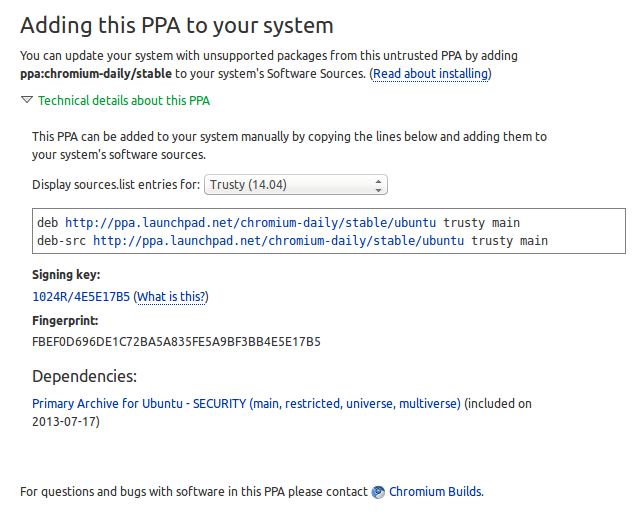
\includegraphics[scale=0.5]{pics/37.png}
\end{center}

در این صفحه اطلاعاتی در مورد آدرس \lr{ppa} نشان داده می‌شود. می‌توان \lr{ppa} را مانند مخزنی عادی به فایل \lr{\texttt{/etc/apt/sources.list}} اضافه کرد، اما در نسخه‌های اخیر اوبونتو ابزاری برای اضافه‌کردن مستقیم \lr{ppa} از راه ترمینال (یا رابط گرافیکی آن) گنجانده شده است. کافی است که دستور \lr{\texttt{sudo add-apt-repository ppa:ppa-address}} را در ترمینال وارد کنید. بعد از واردکردن دستور، کمی صبر کنید تا تأییدیهٔ افزودن مخزن ظاهر شود. برای تایید آن، کلید \lr{Enter} را فشار دهید و باز هم صبر کنید تا مخزن همراه کلید آن به مجموعهٔ مخازن سیستم‌تان افزوده شود. مدت زمان این عملیات کاملاً به سرعت و وضعیت اینترنت‌تان بستگی دارد.

\subsection[نرم‌افزار گرافیکی Synaptic]{نرم‌افزار گرافیکی \lr{Synaptic}}
در صورتی که با استفاده از \lr{Ubuntu Software Center} احساس می‌کنید روی سیستم کنترل کافی ندارید و استفاده از \lr{apt} هم برای‌تان سخت است، می‌توانید از \lr{Synaptic} استفاده کنید. \lr{Synaptic} در واقع رابطی گرافیکی برای \lr{apt} است. با استفاده از سیناپتیک می‌توانید تک‌تک نرم‌افزارها و کتاب‌خانه‌های موجود در مخازن اضافه‌شده به اوبونتوتان را مشاهده کنید.\\
\lr{Synaptic} در نسخه‌های قدیمی اوبونتو جزو نرم‌افزارهای پیش‌فرض اوبونتو بود، اما در نسخه‌های اخیر، با اضافه‌شدن \lr{Ubuntu Software Center}، سیناپتیک از نرم‌افزارهای پیش‌فرض اوبونتو حذف شد. برای همین باید آن را با استفاده از \lr{apt} یا \lr{USC} نصب کنید.

\begin{center}
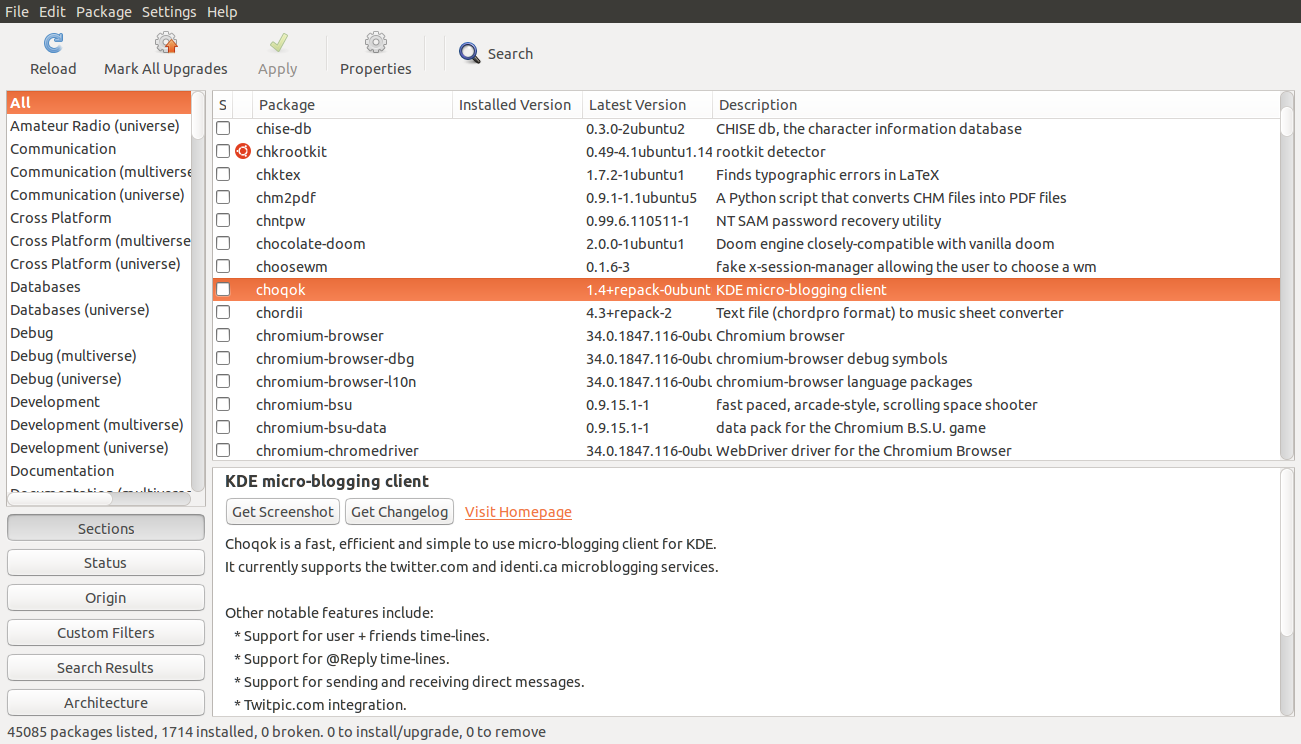
\includegraphics[scale=0.37]{pics/38.png}
\end{center}


\subsection[dpkg]{\lr{dpkg}}
\lr{dpkg} در واقع برنامهٔ اصلی حذف و نصب نرم‌افزار در دبیان است و همهٔ نرم‌افزارهایی که در این بخش معرفی شدند، برای نصب نرم‌افزار از \lr{dpkg} استفاده می‌کنند. دلیل معرفی آن در انتهای این بخش، کاربرد نسبتاً کم آن برای کاربران عادی است. تنها زمانی به استفاده از خود \lr{dpkg} نیاز پیدا می‌کنید که بخواهید فایل با پسوند \lr{.deb} یک نرم‌افزار را دستی نصب کنید.\\

\subsubsection[پارامترهای dpkg]{پارامترهای \lr{dpkg}}
\lr{dpkg} دارای پارامترهای زیادی است. در این‌جا تنها به دو تای آن اشاره می‌شود.

\begin{description}
\item[نصب]: \lr{\texttt{sudo dpkg -i package.deb}}
\item[حذف]: \lr{\texttt{sudo dpkg -r package}}
\end{description}

\subsubsection[gdebi]{\lr{gdebi}}
\lr{gdebi} یک رابط گرافیکی برای نصب بسته‌های \lr{.deb} است (البته امکان استفاده از آن در ترمینال نیز وجود دارد). مزیت استفاده از \lr{gdebi} به جای \lr{dpkg} (علاوه بر گرافیکی‌بودن آن)، دانلودکردن و نصب همهٔ وابستگی‌های نرم‌افزاری مورد نیاز است. در صورتی که نیازمندی‌های یک بستهٔ \lr{.deb} را نصب نکرده باشید و بسته را با \lr{dpkg} نصب کنید، مدیر بسته‌های سیستم آسیب می‌بیند. این وضعیت به دلیلی که گفته شد، در \lr{gdebi} وجود ندارد.\\
برای نصب \lr{gdebi} کافی است که بستهٔ \lr{gdebi} را از مخازن دریافت و نصب کنید. بعد از نصب آن، روی بستهٔ \lr{.deb} ای که می‌خواهید نصب کنید، راست‌کلیک کنید و \lr{gdebi} را انتخاب کنید.

\begin{center}
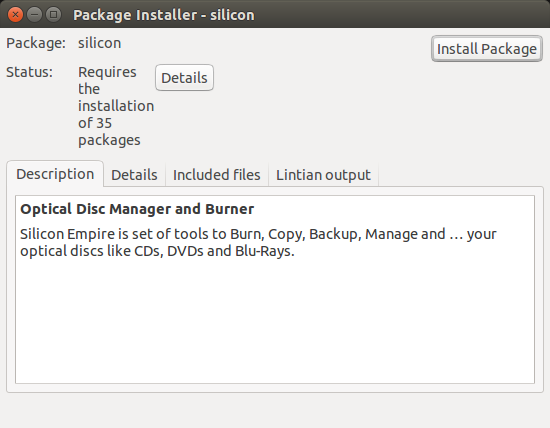
\includegraphics[scale=0.5]{pics/39.png}
\end{center}

\chapter{نرم‌افزارهای اوبونتو}
در این بخش، به معرفی برترین و کاربردی‌ترین نرم‌افزارهای اوبونتو می‌پردازیم و توضیح مختصری راجع به هر یک از نرم‌افزارها ارائه می‌کنیم. لازم به ذکر است که تمامی نرم‌افزارهای زیر، آزاد، متن‌باز و رایگان بوده و شما می‌توانید این نرم‌افزارها را به راحتی و با جست‌و‌جو در \lr{Software Center} نصب کنید.


\section{نرم‌افزارهای برتر}
\subsection[LibreOffice]{\lr{LibreOffice}}
لیبره‌آفیس یکی از اولین نیازمندی‌های یک کاربر متوسط است. این بستهٔ نرم‌افزاری جایگزین مناسبی برای نرم‌افزار آفیس مایکروسافت است.
\begin{center}
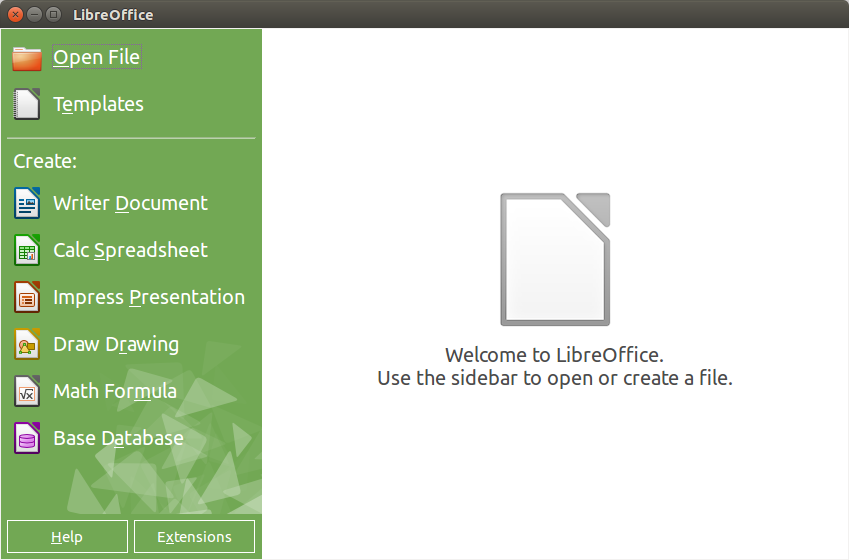
\includegraphics[scale=0.46]{pics/40.png}
\end{center}

لیبره آفیس از بخش‌های زیر تشکیل می‌شود:
\begin{itemize}
\item \lr{\textbf{Writer}}: برنامه‌ای است برای نوشتن و ویرایش متن. این نرم‌افزار زبان فارسی را کاملاً پشتیبانی می‌کند. خروجی پیش‌فرض آن \lr{odt} است، اما می‌توانید خروجی‌هایی مانند \lr{doc} و \lr{pdf} نیز داشته باشید.
\item \lr{\textbf{Impress}}: نرم‌افزار ساخت فایل‌های ارائه که معادل \lr{PowerPoint} در مجموعهٔ آفیس مایکروسافت است.
\item \lr{\textbf{Calc}}: این نرم‌افزار برای ساخت و ویرایش فایل‌های صفحه‌گسترده است.
\item \lr{\textbf{Draw}}: برای طراحی‌های سادهٔ گرافیکی مورد استفاده قرار می‌گیرد.
\item \lr{\textbf{Base}}: نرم افزاری برای طراحی مفهومی پایگاه‌داده و روابط بین جداول است و عملکردی مانند \lr{MS Access} و \lr{Power Designer} دارد.
\item \lr{\textbf{Math}}: کار نوشتن فرمول‌های ریاضی را انجام می‌دهد.
\end{itemize}

\subsection[Gimp]{\lr{Gimp}}

\begin{center}
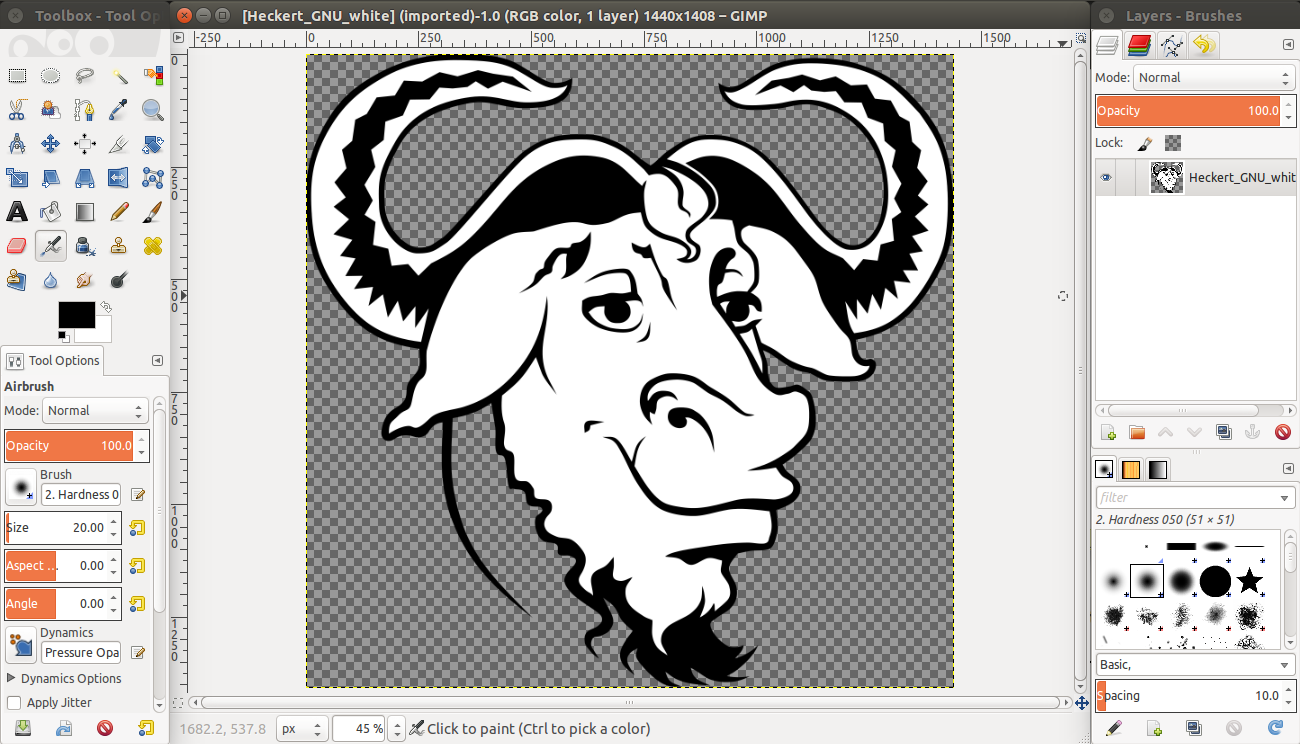
\includegraphics[scale=0.36]{pics/41.png}
\end{center}

نرم‌افزاری است که برای طراحی‌های گرافیکی و ویرایش تصاویر استفاده می‌شود و تا حدودی شبیه \lr{Photoshop} است. از فایل‌های \lr{psd} نیز پشتیبانی می‌کند. \lr{Gimp} ابزارها و فیلترهای متنوعی برای ویرایش تصاویر دارد که به ساخت تصاویری زیبا کمک می‌کند.

\subsection[Inkscape]{\lr{Inkscape}}

\begin{center}
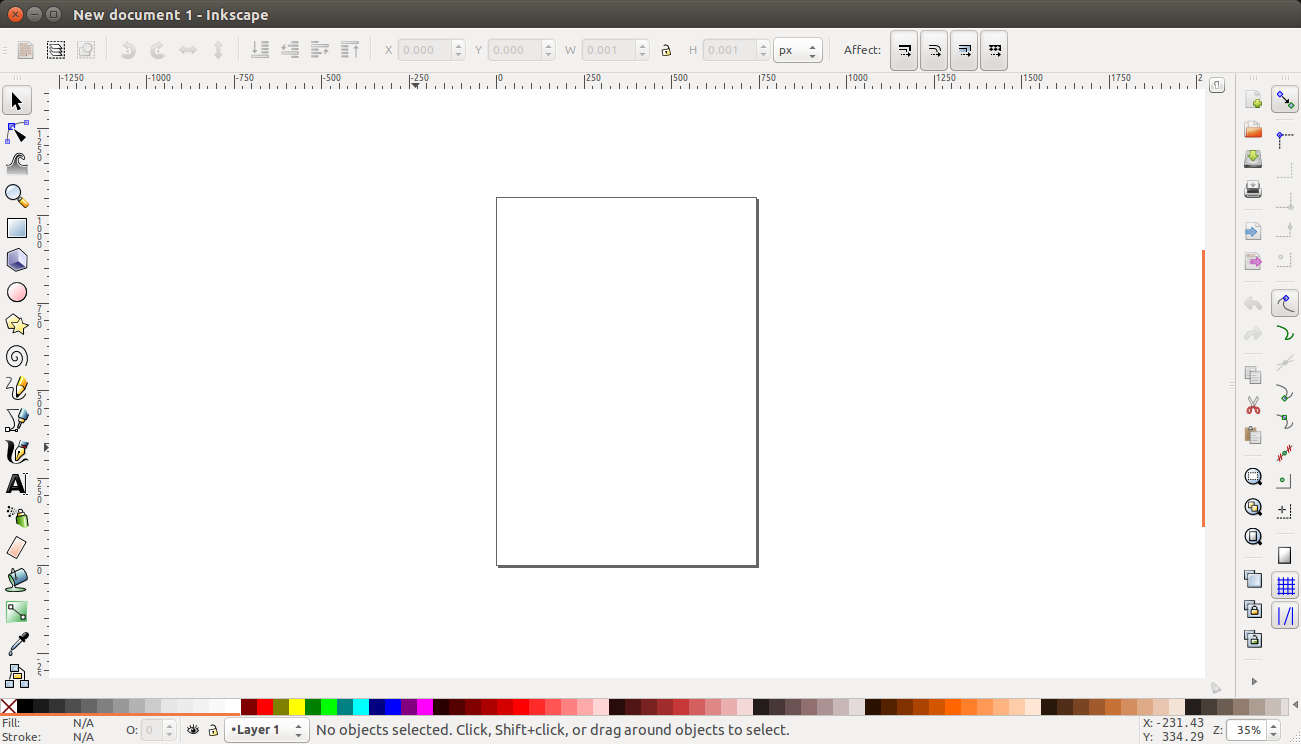
\includegraphics[scale=0.3]{pics/42.png}
\end{center}

یکی از حرفه‌ای‌ترین نرم‌افزارها در زمینه طراحی تصاویر بُرداری (\lr{vector}) است. بسیاری از طرح‌ها و آیکن‌های موجود در اوبونتو با این نرم‌افزار طراحی شده‌اند. \lr{Inkscape} جایگزین مناسبی برای نرم‌افزار \lr{illustrator} به حساب می‌آید.

\subsection[Blender]{\lr{Blender}}

\begin{center}
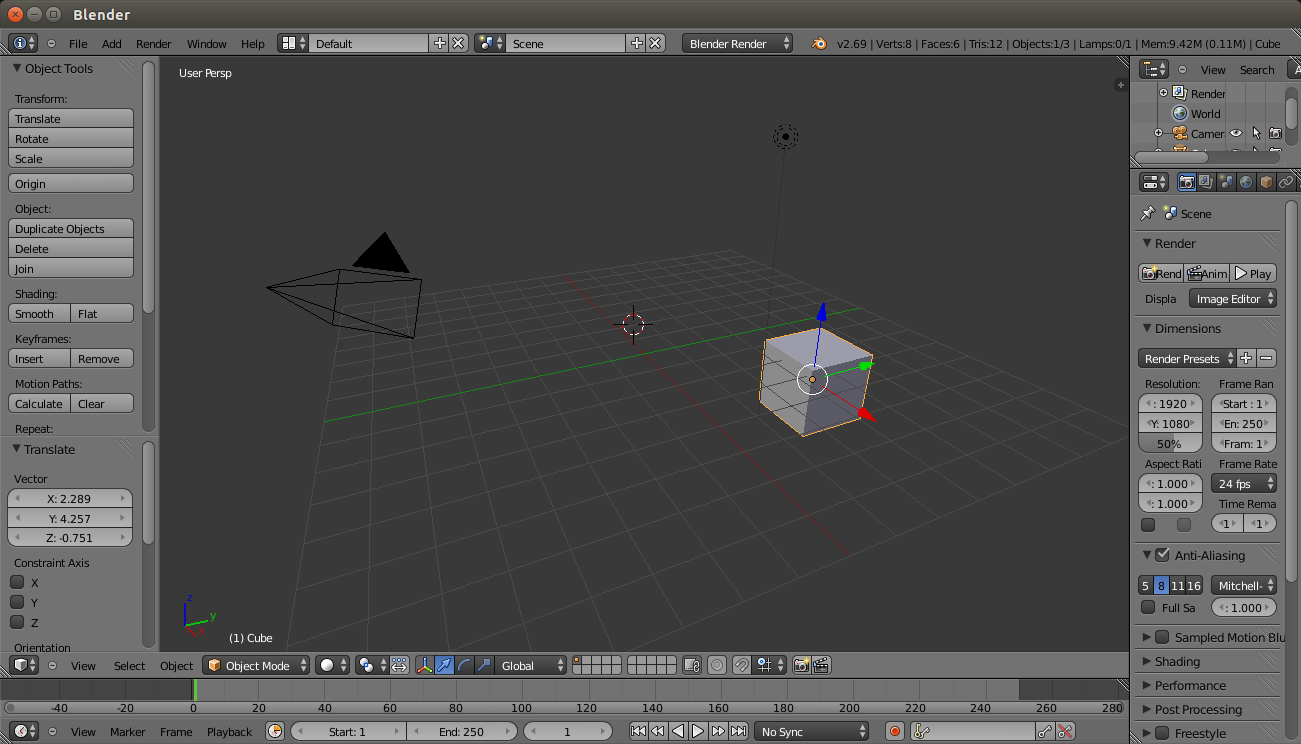
\includegraphics[scale=0.3]{pics/43.png}
\end{center}

این نرم‌افزار برای تمامی طراحان سه‌بعدی دنیای کامپیوتر توصیه می‌شود. \lr{Blender} نرم‌افزاری است که در بسیاری از فیلم‌های هالیوودی و بازی‌های کامپیوتری معروف استفاده شده است و همچنین انیمیشن‌های زیادی با این نرم‌افزار ساخته شده است.

\subsection[K3b]{\lr{K3b}}

\begin{center}
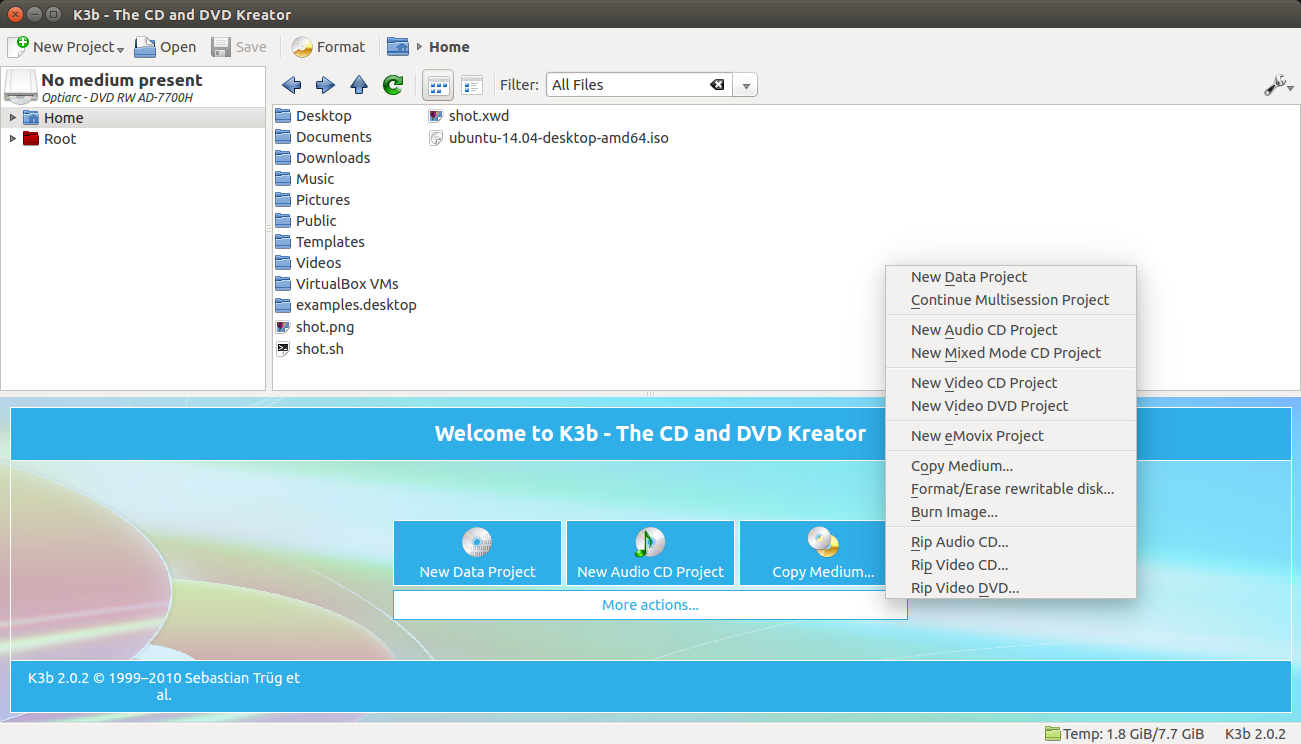
\includegraphics[scale=0.3]{pics/44.png}
\end{center}

نرم‌افزاری برای کپی‌برداری از \lr{CD} و \lr{DVD} است. \lr{K3b} بدون شک یکی از بهترین نرم‌افزارهای موجود در این زمینه است.

\subsection[Darktable]{\lr{Darktable}}

\begin{center}
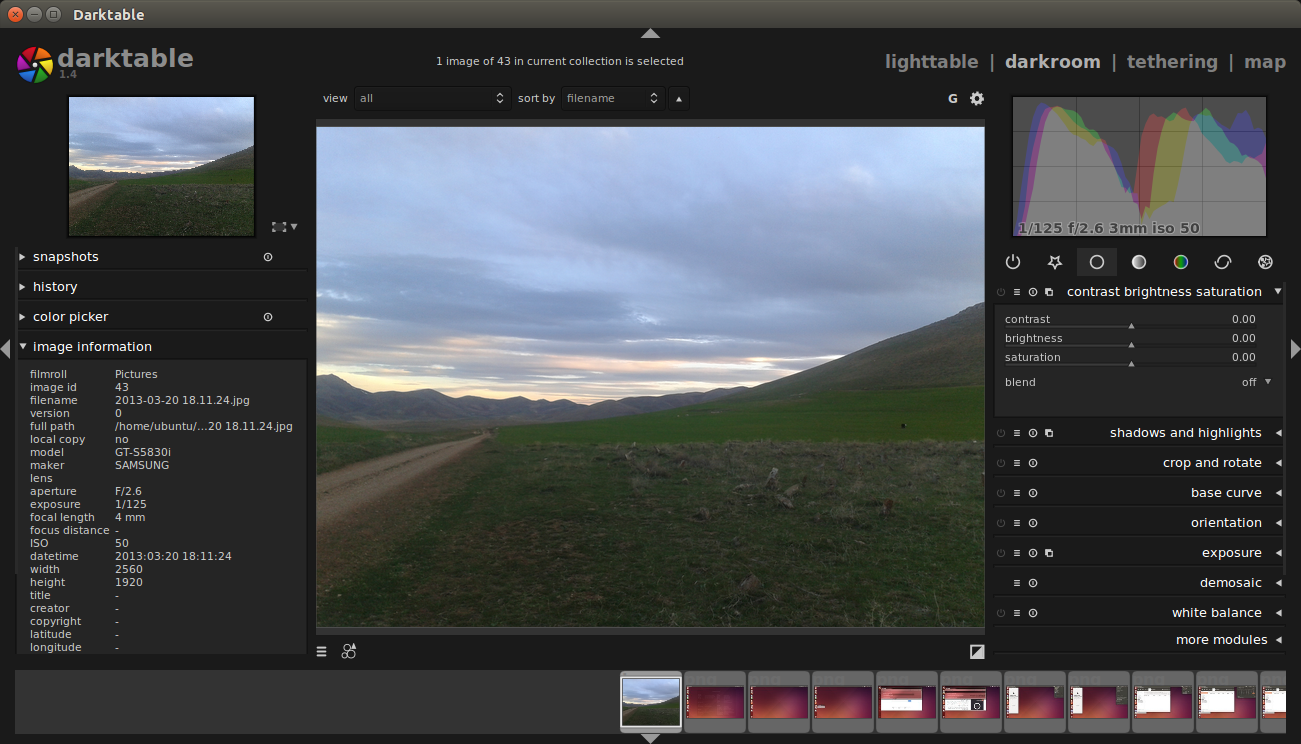
\includegraphics[scale=0.3]{pics/45.png}
\end{center}

چه یک عکاس حرفه‌ای باشید و چه یک کاربر سادهٔ کامپیوتر، با عکس سر و کار خواهید داشت. مهم نیست این عکس‌ها با دوربین حرفه‌ای گرفته می‌شوند یا با دوربین تلفن‌همراه‌تان، مهم نیست که این عکس‌ها از دل طبیعت گرفته شده‌اند یا عکس‌هایی خانوادگی هستند؛ تمامی این عکس‌ها احتیاج به مدیریت و ویرایش در میزان رنگ و روشنی تصویر یا تغییراتی از این دست دارند. \lr{Darktable} تمامی چنین نیازهایی را پاسخ خواهد داد.

\subsection[Virtualbox]{\lr{Virtualbox}}

\begin{center}
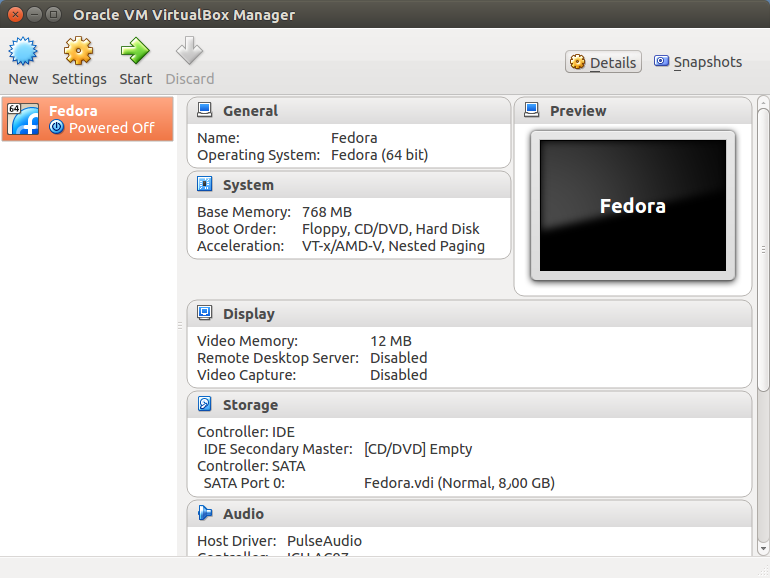
\includegraphics[scale=0.4]{pics/46.png}
\end{center}

با کمک این نرم‌افزار شما قادر خواهید بود که در اوبونتو سیستم‌عامل دیگری مانند ویندوز را نصب کنید و با اختصاص منابع سیستمی به آن، می‌توانید کاملاً از آن سیستم‌عامل و نرم‌افزارهایی که روی آن نصب کرده‌اید، استفاده کنید.

\subsection[Wine]{\lr{Wine}}

\begin{center}
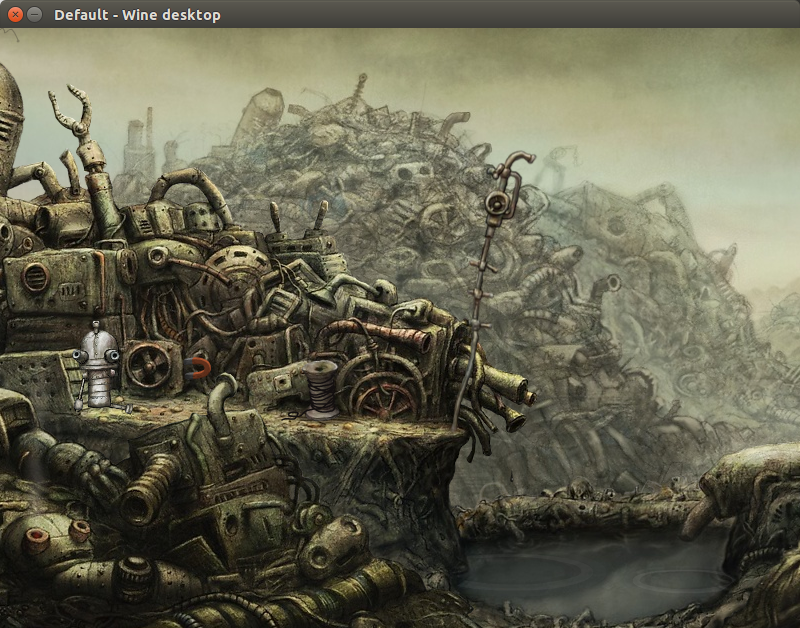
\includegraphics[scale=0.4]{pics/47.png}
\end{center}

معمولاً در اوایل دوران کوچ به سیستم‌عامل دیگر، زمان‌هایی پیش می‌آید که به نرم‌افزارهای سیستم‌عامل قبلی خود نیاز پیدا کنید و به دلیل آشنا نبودن با نرم‌افزارهای جایگزین موجود، شاید در ابتدا کار با سیستم‌عامل جدید کمی آزار‌دهنده باشد. \lr{Wine} نرم‌افزاری است که به شما امکان اجرای بسیاری از نرم‌افزارها و بازی‌های سیستم‌عامل ویندوز را روی اوبونتو می‌دهد.

\subsection[Goldendict]{\lr{Goldendict}}

\begin{center}
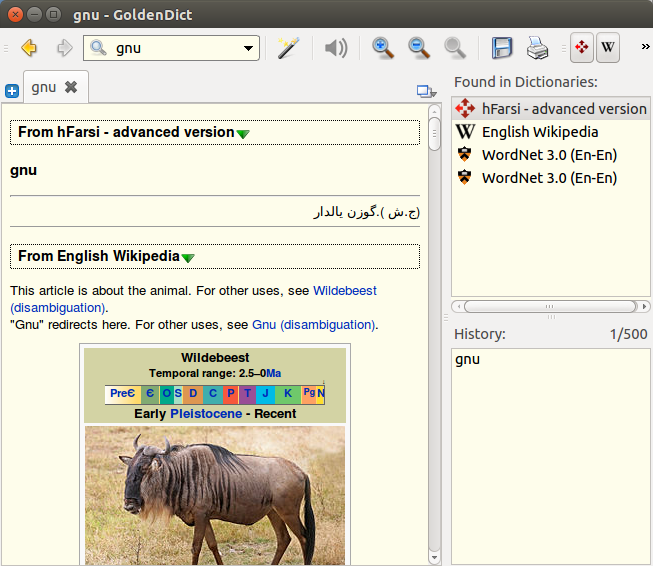
\includegraphics[scale=0.39]{pics/48.png}
\end{center}

وجود یک واژه‌نامه در رایانه نیازی است که کاربران کم‌سن‌وسال تا استادان زبان را شامل می‌شود. \lr{Goldendict} یک برنامهٔ تمام‌عیار برای این نیاز است. این برنامه از کتاب‌خانه لغات \lr{Babylon} با قالب \lr{bgl} نیز پشتیبانی می‌کند.

\subsection[VLC]{\lr{VLC}}

\begin{center}
\includegraphics[scale=0.39]{pics/49.png}
\end{center}

شاید با \lr{VLC} در سیستم‌عامل‌های دیگر نیز کار کرده باشید. \lr{VLC} در زمینهٔ پخش فایل‌های موسیقی و ویدیویی همه‌فن‌حریف است و از بیش‌تر فرمت‌ها، از \lr{MP3} گرفته تا \lr{Bluray}، پشتیانی می‌کند.

\section{نرم‌افزارهای معادل}
از تمام مزایای لینوکس مثل آزادی که بگذریم، شما در گنو/لینوکس هم باید کارهای متداول خود را انجام بدهید. در لیست زیر، نرم‌افزارهای گنو/لینوکسی معادل نرم‌افزارهای پرکاربرد در ویندوز و \lr{Mac OS X} معرفی می‌شوند.\\

\begin{table}[ht]
\caption{لیست نرم‌افزارهای معادل}
\centering
\begin{tabular}{|c|c|}
\hline
\textbf{\lr{\Large Ubuntu}} & \textbf{\lr{\Large Windows / Mac OS X}} \\[1ex]
\hline
\lr{Pinta} & \lr{Paint}\\
\hline
\lr{VLC} & \lr{KMPlayer}\\
\hline
\lr{Totem} & \lr{Windows Media Player}\\
\hline
\lr{Gimp} & \lr{Photoshop}\\
\hline
\lr{OpenShot, PiTiVi} & \lr{Windows Media Player}\\
\hline
\lr{Rhythmbox, Noise} & \lr{iTunes}\\
\hline
\lr{gedit} & \lr{Windows Notepad}\\
\hline
\lr{Blender} & \lr{Autodesk 3D Max}\\
\hline
\lr{LibreCAD} & \lr{Autodesk AutoCAD}\\
\hline
\lr{Audacious} & \lr{Winamp}\\
\hline
\lr{Evince} & \lr{Adobe Acrobat Reader}\\
\hline
\lr{Inkscape} & \lr{Adobe Illustrator}\\
\hline
\lr{Scribus} & \lr{Adobe InDesign}\\
\hline
\lr{LibreOffice} & \lr{Microsoft Office, Apple iWork}\\
\hline
\lr{Empathy, Pidgin} & \lr{Yahoo Messenger, Google Talk}\\
\hline
\end{tabular}
\end{table}

\chapter{کار با ترمینال}
از زیرمجموعه‌های لینوکس رابط‌های گرافیکی یا \lr{GUI}ها هستند (\lr{Graphical User Interface}) که شما در آن می‌توانید موس‌تان را تکان دهید، کلیک کنید و بکشید، و می‌توانید بدون این‌که مستندات زیادی را بخوانید، کارهای‌تان را انجام دهید. محیط سنتی \lr{Unix} یک رابط خط فرمان یا \lr{CLI} است (\lr{Command Line Interface}) که دستورات را در آن تایپ می‌کنید تا به کامپیوتر بگویید که چه کاری انجام دهد. این روش خیلی سریع‌تر و قدرتمندتر است، اما لازم است که دستورات را بشناسید. در برخی شرایط، مخصوصا هنگام پیکربندی سیستم، مجبوریم که از ترمینال استفاده کنیم.

\section{آشنایی اولیه با ترمینال}
برای بازکردن ترمینال در اوبونتو کافی است که روی لانچر کلیک کنید و چند حرف از کلمهٔ \lr{Terminal} را تایپ کنید تا آیکن ترمینال ظاهر شود. روی آن کلیک کنید. پنجرهٔ ترمینال باز خواهد شد.

\begin{center}
\includegraphics[scale=0.48]{pics/50.png}
\end{center}

در پنجرهٔ بازشده، یک خط مثل \lr{\texttt{ubuntu@ubuntu-book:$\sim$\$}} را مشاهده می‌کنید. \lr{\texttt{ubuntu}} نام کاربری کنونی‌تان، \lr{\texttt{ubuntu-book}} نام رایانهٔ‌تان، \lr{\texttt{$\sim$}} محل پوشهٔ کنونی‌تان (که این علامت، به معنی پوشهٔ خانگی‌تان است) و \lr{\texttt{\$}} هم به معنی دارابودن مجوز عادی و نداشتن مجوز کاربر ریشه است.

\section[،sudo اجرای دستورات با بالاترین مجوز دسترسی]{\lr{sudo}، اجرای دستورات با بالاترین مجوز دسترسی}
بعضی از دستورات به اضافه‌کردن دستور \lr{\texttt{sudo}} (\lr{Super User Do}) به اول‌شان نیاز دارند. این در صورتی است که با فایل‌ها و پوشه‌هایی کار کنید که متعلق به حساب کاربری شما نباشد. این یک دستور ویژه است که به صورت موقت به شما اجازهٔ تغییر تنظیمات کامپیوتر را می‌دهد. پس از واردکردن این دستور، ترمینال از شما گذرواژه را خواهد پرسید. می‌بینید که با واردکردن گذرواژه چیزی در ترمینال نشان داده نمی‌شود. این کار برای امنیت بیش‌تر است.

\subsection[تفاوت sudo با su]{تفاوت \lr{sudo} با \lr{su}}
در بسیاری از گنو/لینوکس‌های دیگر، امکان استفاده از دستور \lr{\texttt{sudo}} به صورت پیش‌فرض وجود ندارد. در این توزیع‌ها، به جای \lr{\texttt{sudo}} از \lr{\texttt{su}} استفاده می‌شود.\\
\lr{\texttt{su}} مخفف عبارت \lr{Substitute User} به معنای «تغییر کاربر» است. یعنی علاوه بر تغییر کاربر کنونی به کاربر ریشه (کاربر ریشه یا \lr{root}، دارای بالاترین مجوز در سیستم‌های یونیکسی است)، می‌توان با واردکردن دستور \lr{\texttt{su \emph{user}}} (که به جای \lr{\texttt{\emph{user}}} باید نام کاربر مورد نظر را بنویسید)، به عنوان آن کاربر فعالیت کرد. دستور \lr{\texttt{su}} هم وارد حساب کاربری ریشه خواهد شد. با زدن این دستور، خط ترمینال شبیه \lr{\texttt{root@ubuntu-book:/home/ubuntu\#}} خواهد شد. علامت \lr{\texttt{\#}} نشان‌دهندهٔ حضور در حساب کاربری ریشه است.\\
در اوبونتو، امکان استفاده از \lr{\texttt{su}} هم وجود دارد. می‌توان با دستور \lr{\texttt{sudo su}}، وارد حساب کاربری ریشه شد. برای فعال‌کردن \lr{\texttt{su}}، باید ابتدا برای کاربر ریشه گذرواژه‌ای را با دستور \lr{\texttt{sudo passwd root}} تعریف کنید. سپس می‌توانید با زدن \lr{\texttt{su}} و واردکردن گذرواژهٔ ریشه، بالاترین مجوزها را داشته باشید.\\
استفاده از دستورهای \lr{\texttt{su}} و \lr{\texttt{sudo su}} به هیچ وجه برای افراد تازه‌کار توصیه نمی‌شود. با داشتن مجوز ریشه و با زدن دستورهای نابه‌جا، امکان از بین رفتن اطلاعات و تنظیمات‌تان وجود دارد.\\
برای خارج‌شدن از ترمینال کاربر، کلمهٔ \lr{\texttt{exit}} را وارد کنید.

\section{دستورهای پرکاربرد ترمینال}
\subsection{دستورهای مربوط به کار با پرونده‌ها و پوشه‌ها}
\begin{itemize}
\item \textbf{\texttt{\Large pwd}}: این دستور به شما این امکان را می‌دهد که بدانید درچه پوشه‌ای هستید (\lr{pwd} مخفف عبارت \lr{Print Working Directory} است).  این اطلاعات را در نوار عنوان پنجره هم نشان داده می‌شود.

\item \textbf{\texttt{\Large ls}}: دستور \lr{\texttt{ls}} به شما پرونده‌های درون پوشه‌ای را که در آن هستید، نشان می‌دهد که اگر با بعضی انتخاب‌های دیگر (\lr{Options}) به کار رود، می‌توانید حجم پرونده‌ها، زمان و مکان ساخته‌شدن و مجوز دسترسی آن‌ها را مشاهده کنید. مثلاً \lr{\texttt{ls $\sim$}}، به شما پرونده‌های درون پوشهٔ \lr{home}تان را نشان می‌دهد.

\item \textbf{\texttt{\Large cd}}: دستور \lr{\texttt{cd}} به شما اجازهٔ عوض‌کردن پوشهٔ کنونی را می‌دهد. هنگامی که یک ترمینال را باز می‌کنید، شما در پوشهٔ \lr{home}تان هستید. برای جابه‌جایی میان پوشه‌های سیستم دستور \lr{\texttt{cd}} را به کار ببرید.\\
برای عقب‌رفتن به اندازهٔ یک پوشه، از \lr{\texttt{cd ..}} و برای برگشت به پوشهٔ پیشین، از \lr{\texttt{cd -}} استفاده کنید.

\item \textbf{\texttt{\Large cp}}: دستور \lr{\texttt{cp}} یک رونوشت از پرونده را برای شما می‌سازد. برای مثال، \lr{\texttt{cp file foo}} یک کپی دقیق از \lr{\texttt{file}} را می‌سازد و نام آن را به \lr{\texttt{foo}} تغییر می‌دهد، اما پروندهٔ \lr{\texttt{file}} هنوز در محل خودش قرار دارد. اگر می‌خواهید از یک پوشه کپی‌ای داشته باشید، باید از دستور \lr{\texttt{cp -r directory foo}} استفاده کنید.

\item \textbf{\texttt{\Large mv}}: دستور \lr{\texttt{mv}} یک فایل را به مکانی دیگر منتقل می کند یا نام آن را تغییر می‌دهد. دستور \lr{\texttt{mv file foo}}، نام فایل \lr{\texttt{file}} را به \lr{\texttt{foo}} تغییر می دهد. \lr{\texttt{mv foo \texttt{$\sim$}/Desktop}} فایل \lr{\texttt{foo}} را به پوشهٔ دسکتاپ شما منتقل می‌کند، اما نام آن را تغییر نمی‌دهد.


\item \textbf{\texttt{\Large rm}}: این دستور برای حذف‌کردن و برداشتن فایل‌ها به کار می‌رود. با قراردادن آپشن \lr{\texttt{-r}}، مانند \lr{\texttt{rm -r ~/Desktop/1/}}، می‌توان دستور را برای حذف پوشه‌ها هم به کار برد.

\item \textbf{\texttt{\Large mkdir}}: دستور \lr{\texttt{mkdir}} به شما اجازهٔ ساخت پوشه را می‌دهد. مثلاً \lr{\texttt{mkdir Music}} یک پوشه به نام \lr{\texttt{Music}} را خواهد ساخت.

\item \textbf{\texttt{\Large grep}}: از این دستور برای جست‌وجوی عبارات در پرونده‌ها یا خروجی دستورات دیگر استفاده می‌شود (به صورت \lr{\texttt{grep [-options] pattern [filename]}}). این دستور دو حالت دیگر نیز دارد؛ \lr{\texttt{fgrep}} برای لیست‌کردن خطوط دارای عبارات موردنظر (معادل \lr{\texttt{grep -f}}) و \lr{\texttt{egrep}} که برای یک الگو در فایل می‌گردد (معادل \lr{\texttt{grep -e}}).\\\\
برخی از انتخاب‌های این دستور:
\begin{description}
\item[\lr{\texttt{-w}}] دقیقاً به دنبال کلمهٔ موردنظر می‌گردد. مثلاً \lr{\texttt{grep -w it myfile}}، دقیقاً به دنبال \lr{\texttt{it}} می‌گردد و مثلاً \lr{\texttt{item}} را در نتایج جست‌وجو نشان نمی‌دهد.

\item[\lr{\texttt{-i}}] فرمان \lr{\texttt{grep}} نسبت به بزرگی و کوچکی حروف حساس است. با آپشن \lr{\texttt{-i}} این حساسیت از بین می‌رود.

\item[\lr{\texttt{-v}}] برای لیست‌کردن تمام خطوطی که کلمهٔ موردنظر را ندارند، استفاده می‌شود. همراه \lr{\texttt{fgrep}} به کار می‌رود.

\item[\lr{\texttt{-f}}] در صورتی که یک فایل از کلمات موردنظرتان برای جست‌وجو را بسازید، با به کار بردن این انتخاب همراه \lr{\texttt{fgrep}}، به صورت \lr{\texttt{fgrep -f secondfile myfile}}، می‌توانید خطوطی که هر کدام از این کلمات را دارند، مشخص کنید.
\end{description}
\end{itemize}

\subsection{دستورهایی برای آگاهی از اطلاعات سیستم}
\begin{itemize}
\item \textbf{\texttt{\Large df}}: دستور \lr{\texttt{df}} فضای استفاده‌شدهٔ فایل‌سیستم همهٔ پارتیشن‌های ماونت‌شده را نشان می‌دهد. \lr{\texttt{df -h}} تقریباً بیش‌ترین استفاده را دارد. این دستور از \lr{megabyte} و \lr{gigabyte} به‌جای \lr{block}ها برای گزارش‌دادن استفاده می‌کند (\lr{\texttt{-h}} به معنای «\lr{Human Readable}» است).

\item \textbf{\texttt{\Large du}}: دستور \lr{\texttt{du}} مقدار فضای اشغال‌شده توسط یک پوشه را نشان می‌دهد. این دستور می‌تواند فضای اشغال‌شده توسط تمام زیرپوشه‌ها یا تمام فضای پوشه‌ای را که در آن هستید، نشان دهد. این دستور نیز با آپشن \lr{\texttt{-h}} کار می‌کند.

\item \textbf{\texttt{\Large free}}: دستور \lr{\texttt{free}} مقدار فضای آزاد و استفاده‌شدهٔ حافظهٔ سیستم را نشان می دهد. \lr{\texttt{free -m}} اطلاعات را براساس مگابایت ارائه می دهد.

\item \textbf{\texttt{\Large top}}: دستور \lr{\texttt{top}}، اطلاعات روی سیستم لینوکس شما، پروسه‌های درحال اجرا و وسایل سیستم را نشان می دهد که شامل \lr{CPU} و \lr{RAM} و میزان استفاده از فضای \lr{Swap} و تعداد برنامه‌های درحال اجراست. برای خارج‌شدن از \lr{\texttt{top}} کلید \lr{q} را فشار دهید.

\item \textbf{\texttt{\Large uname}}: مخفف عبارت \lr{unix name} است و نام و نسخه و برخی خصوصیات دیگر در مورد رایانه و سیستم‌عامل را نشان می‌دهد. این دستور حتماً باید با آپشن‌های آن همراه شود. این آپشن‌ها در زیر آورده شده‌اند.
\begin{description}
\item[\lr{\texttt{-a}}] تمام اطلاعات ممکن را نشان می‌دهد.

\item[\lr{\texttt{-r}}] نسخهٔ هستهٔ لینوکس‌تان را نشان می‌دهد.

\item[\lr{\texttt{-p}}] برای تعیین نوع پردازنده (۳۲ یا ۶۴ بیت بودن) به کار می‌رود.
\end{description}

\item \textbf{\texttt{\Large ifconfig}}: رابط‌های شبکهٔ سیستم‌تان را به شما گزارش می‌کند.

\item \textbf{\texttt{\Large killall}}: این دستور تمام پروسه‌های برنامهٔ موردنظر را متوقف می‌کند. انتخاب \lr{\texttt{-i}}، قبل از توقف هر پروسه، از شما تأییدکردن آن را درخواست می‌کند.

\item \textbf{\texttt{\Large shutdown}}: امکان خاموش یا ری‌استارت‌کردن رایانه را به شما می‌دهد. این دستور باید به شکل \lr{\texttt{shutdown [option] [time]}} به کار رود. برخی انتخاب‌های این دستور عبارت‌اند از:
\begin{description}
\item[\lr{\texttt{-h}}] برای خاموش‌کردن سیستم به کار می‌رود.

\item[\lr{\texttt{-r}}] رایانه را ری‌استارت می‌کند.

\item[\lr{\texttt{-c}}] یک دستور \lr{\texttt{shutdown}} در حال اجرا را لغو می‌کند.
\end{description}
برای واردکردن زمان هم ۳ شکل وجود دارد:
\begin{description}
\item[\lr{\texttt{now}}]: اجرای بلافاصلهٔ دستور

\item[\lr{\texttt{hour:min}}]: مثلاً \lr{\texttt{21:40}}

\item[\lr{\texttt{+m}}]: به جای \lr{\texttt{m}} تعداد دقایق موردنظر تا اجرای دستور را وارد کنید.
\end{description}
برای اجرای دستور، حتماً باید کاربر ریشه باشید.

\item \textbf{\texttt{\Large man}}: مسلماً بسیاری از افراد از نحوهٔ کارکردن و آپشن‌های دستورهای مختلف آگاه نیستند. برای اطلاع از این‌ها می‌توان از اینترنت استفاده کرد. اما راه دیگری هم وجود دارد که احتیاجی هم به اینترنت ندارد: دستور \lr{\texttt{man}}.\\
دستور \lr{\texttt{man}} در حقیقت جستجوگر فایل‌های راهنمای برنامه‌هاست. بسیاری از برنامه‌های لینوکسی همراه خود فایل‌های راهنما دارند که با \lr{\texttt{man}} قابل دسترس‌اند. برای مثال، \lr{\texttt{man man}}، فایل راهنمای \lr{\texttt{man}} را نشان می‌دهد. برای خروج از محیط راهنما، دکمهٔ \lr{Q} را فشار دهید.
\end{itemize}

\section{کلیدهای کاربردی در ترمینال}
\begin{description}
\item[توقف دستور در حال اجرا]: برای این کار کافی است دکمه‌های \lr{Ctrl + C} را بزنید.

\item[چسباندن متن]: کلیدهای \lr{Ctrl + V} در ترمینال کار چسباندن را انجام نمی‌دهند. برای چسباندن متن، می‌بایست کلید \lr{Shift} را نیز فشار دهید؛ یعنی \lr{Ctrl + Shift + V}.

\item[بازکردن زبانهٔ جدید]: از کلیدهای \lr{Ctrl + Shift + T} استفاده کنید.
\end{description}

\chapter{بازی‌های گنو/لینوکس}
گرچه اساساً گنو/لینوکس برای بازی‌کردن به وجود نیامده است، اما به دلیل محبوبیت روزافزون آن میان کاربران غیرحرفه‌ای در سال‌های اخیر، بازی‌های خوبی برای گنو/لینوکس ارائه شده‌اند. هرچند که این بازی‌ها به هیچ عنوان در حد بازی‌های باکیفیت ویندوزی نیستند، اما با توجه به رایگان‌بودن (و در مواردی آزادبودن) آن‌ها قابل قبول‌اند و ارزش امتحان‌کردن دارند. در ادامه بازی‌هایی از انواع سبک‌ها معرفی می‌شوند.

\section{بازی‌های اول شخص}
\subsection[Nexuiz]{\lr{Nexuiz}}

\subsection[Tremulous]{\lr{Tremulous}}
\subsection[Terror Urban]{\lr{Urban Terror}}
\subsection[Warsow]{\lr{Warsow}}
\subsection[OpenArena]{\lr{OpenArena}}

\section{بازی‌های استراتژیک}
\subsection[Freeciv]{\lr{Freeciv}}
\subsection[2100 Warzone]{\lr{Warzone 2100}}
\subsection[OpenTTD]{\lr{OpenTTD}}
\subsection[FreeCol]{\lr{FreeCol}}

\section{بازی‌های مسابقه‌ای}
\subsection[TORCS]{\lr{TORCS}}
\subsection[Racer Tux]{\lr{Tux Racer}}

\section{بازی‌های نقش‌آفرینی}
\subsection[Auteria]{\lr{Auteria}}
\subsection[PlaneShift]{\lr{PlaneShift}}


\section{بازی‌های آموزشی}
\subsection[gbrainy]{\lr{gbrainy}}

\section[بازی‌های Steam]{بازی‌های \lr{Steam}}

\include{chapter9}
%\include{Appendix} %درج پیوست‌ها

% \include{Resources} %درج منابع و مآخذ
% \include{AbstractEnglish} %درج چکیده‌ی انگلیسی
\include{CoverBack} %درج صفحه‌ی آخر
\end{document} %پایان سند پایان‌نامه
